
%\chapter{Vision, Action and World Models}\label{chap:world}
\chapter{视觉、动作与世界模型}\label{chap:world}

\begin{learningbox}
智能体所处的世界不止由语言构成。在本章中，你将学习基于 Transformer 的模型如何在语言之外的模态中获得世界知识。
具体来说，你将能够：
\begin{itemize}[leftmargin=*, nosep]
    \item 描述{\em 视觉—语言模型}（VLM）的架构——这类（大多）Transformer 模型由语言部分与视觉部分组成。VLM 非常成功，例如能生成逼真的假图像与影视片段。

    \item 理解{\em 视觉—语言—动作}模型如何工作。VLA 同样在机器人动作上训练过。VLA 有助于提升机器人行为的通用性。
    
    \item 解释为什么智能体受益于{\em 世界模型}：这类模型学到了我们周围世界的某些物理属性，从而防止智能体试图穿墙而过。%The term {\em world model} is borrowed from the field of {\em model-based reinforcement learning}, where such models are trained from observations in the environment, and then used to efficiently learn optimal action policies.  
\end{itemize}
\end{learningbox}


%*
%- pretraining
%-- vlm
%-- decisions
%-- VLA
%- finetuning
%-- decisions
%-- action

%- vlm
%-- pretraining
%-- finetuning
%- decisions
%-- pretraining
%-- finetuning
%- VLA
%-- pretraining
%-- finetuning

%Todo: read Ch 7 and write contents

%benchmark
%architecture
%learning/code
%results
\begin{comment}
    
%
Agents act, and the LLM should do the reasoning for these actions. To do so, the LLM needs to understand more than just  language. For example, a robotic agent needs to understand which joints to move in its arms. Furthermore, agents may need to be able to interpret spatial or visual data. 

The previous chapter discussed  approaches to improve LLM reasoning by in-context methods. %, a powerful and efficient learning method that does not change the parameters of the underlying transformer model.
%
%, but works purely at the prompt level at inference time. 
To learn other modalities than language, we have to pretrain and finetune the models: we need to go beyond what is possible by in-context learning. 
% , where we do train the parameters of the transformers. 

In this chapter we will shift our focus from language to vision and actions, and our learning methods from in-context learning to  pretraining and finetuning. 
\end{comment}

\section{多模态视觉语言模型}\label{sec:vlm}

%\paragraph{Multi-modal Models}
许多决策都涉及视觉。
正如我们将在本节看到的，%where LLMs are trained on language data, 
Transformer 架构同样能够学习被词元化的视觉模式。在语言与视觉数据上都做过预训练的模型，称为视觉—语言模型（VLM）。VLM 通常由（1）语言部分、（2）视觉部分，以及（3）把两种嵌入结合起来的部分组成。  %In the first section 

我们将讨论这类视觉—语言模型的各种架构。对每一类模型，我们都会描述它的任务、模型架构，以及它所用的训练算法。
我们将看到令人瞩目的结果。

计算机视觉在 AI 中有着漫长而成功的历史。深度学习在图像识别
任务上很早就取得了成功，远早于自然语言
处理的突破 \citep{krizhevsky2012imagenet}。这两个成功领域能否结合起来？这不是一个简单的问题，因为两个领域所依托的深度学习架构颇为不同：图像处理基于卷积神经网络，它在二维矩形像素网格上表现良好；而语言处理基于 Transformer，它在一维词元序列上表现良好。

正如我们将看到的，人们确实已经开发出把这两个领域结合起来的架构，以至于如今大多数前沿模型都是 VLM。%Nevertheless,  a synergy of vision and natural language has been achieved in some architectures. 



\begin{figure}
  \begin{center}
    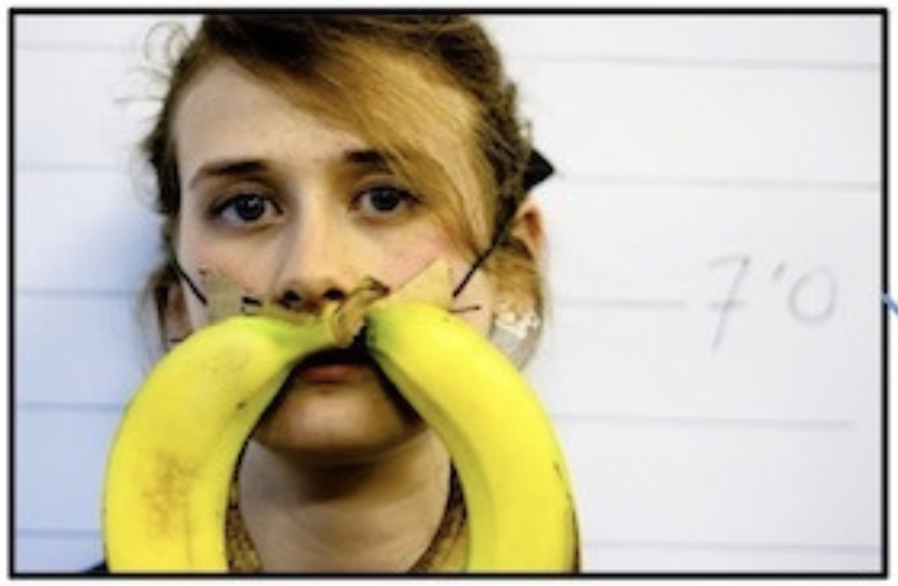
\includegraphics[width=7cm]{figures/VQAbanana}
    \caption{一个视觉问答任务中的问题可能是：{\em 这副胡子是什么做的？}} \label{fig:vqa}  
  \end{center}
\end{figure}

\subsection{任务}
我们先讨论视觉—语言模型必须解决的任务类型，并列出一些流行的基准测试套件。就理解而言，可以在视觉问答（VQA）任务上测试
模型，看它们是否对视觉图像获得了一定的
文字理解。一个相关但属于生成式的任务是图像描述
问题，模型需要为图像生成文字描述。此外，还可以给模型布置图像生成任务。

让我们看几个示例任务。对图~\ref{fig:vqa}，一个 VQA 问题可以是：{\em 这副胡子是什么做的？}，系统应回答：{\em 香蕉}。其他典型的 VQA 问题是统计图像某个区域内某种颜色的某种形状的数量（用来回答诸如：{\em 这个场景里桌子上角有没有一个红色方块？}这样的问题）。这些任务可以非常多样，流行基准也有一批，例如 MOSAIC \citep{burda2025culturally}、GLOBAL-RG \citep{bhatia2024local}、CultureVQA \citep{nayak2024benchmarking}、FoodieQA \citep{li2024foodieqa} 与 MaRVL \citep{liu2021visually}。

%Just benchmarks, or also famous models/approaches, of gaat dat te diep? Nee, dat komt later al.

\begin{figure}
  \begin{center}
    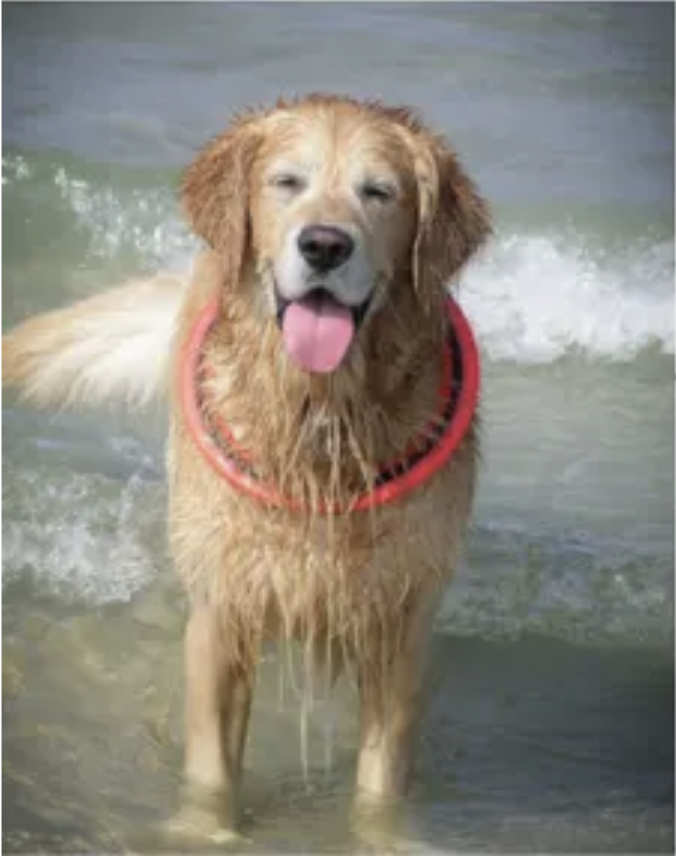
\includegraphics[width=6cm]{figures/captioning}
    \caption{一个图像描述任务，可能的描述是：{\em 一只快乐的狗站在海里}} \label{fig:cap}  
  \end{center}
\end{figure}



在图像描述问题中，可以
提示模型为图~\ref{fig:cap} 中的场景写一句描述，画面显示的是{\em 一只快乐的狗站在海里}。请注意，其他说法同样成立，例如{\em 一只湿漉漉的狗}、{\em 一只很冷的狗}，或{\em 一只戴红项圈的狗站在海里}。流行基准有 MS-COCO \citep{lin2014microsoft}、nocaps\footnote{\url{https://nocaps.org}}，以及面向视频的 MSR-VTT \citep{xu2016msr} 和 VATEX（用于传统的短句描述评估）\citep{wang2019vatex}。更新的基准则聚焦于细致的、多方面的描述：DetailCaps \citep{dong2024benchmarking}、VDC \citep{chai2024auroracap} 与 CapArena \citep{cheng2025caparena}。%\todo{Benchmark overload. Het gaat meer om methoden uit te leggen aan de studenten dan om te laten zien dat ik de literatuur ken. Reduce the }

VLM 的典型应用有摘要、图像生成、搜索与检索、图像分割与目标检测。面向专家级通用智能的大规模多学科多模态理解与推理基准（MMMU）是视觉—语言模型的综合性基准 \citep{yue2024mmmu}。


%!!!!!!!!!!!!!!!!!!!!!!!!!!!!!!!!!!!!!!!

%{\bf REWRITE:} Vision language models are models that can learn
%simultaneously from images and texts to tackle many tasks, from visual
%question answering to image captioning. The use cases include chatting
%about images, image recognition via instructions, visual question
%answering, document understanding, image captioning, and others. Some
%vision language models can also capture spatial properties in an
%image. These models can output bounding boxes or segmentation masks
%when prompted to detect or segment a particular subject, or they can
%localize different entities or answer questions about their relative
%or absolute positions. 

%\url{https://www.ibm.com/think/topics/vision-language-models}
%Goals: 
%- VQA (answer text questions)
%- Captioning (generate text description)
%Applications: Captioning and summarization, Image generation, Image search and retrieval, Image segmentation, Object detection, Visual question answering (VQA)

\subsection{架构}
既然已经看到 VLM 被测试的任务类型，我们该如何设计一个模型来完成这些任务？%Architectures that combine visual and language knowledge should be able to generalize, answer questions, and draw conclusions.

当语言被建模为词元序列时，它是一个顺序的（一维）问题域。当视觉被建模为像素网格时，它是一个矩形的（二维）问题域。相应地，两种应用所用的深度学习架构也不同。对语言，使用 Transformer 架构来发现顺序模式；对图像，使用卷积神经网络来发现二维模式。因此，一个多模态视觉—语言模型该用什么架构并不显然。事实上，当时连 VLM 能否奏效都说不清。

研究最初聚焦于这样一个问题：Transformer 架构是否也能用于图像处理（除了传统的卷积神经网络 CNN 之外）。人们开发出了在图像处理中表现良好的专用视觉 Transformer 与词元化方案 \citep{dosovitskiy2020image}。

\begin{figure}
    \centering
    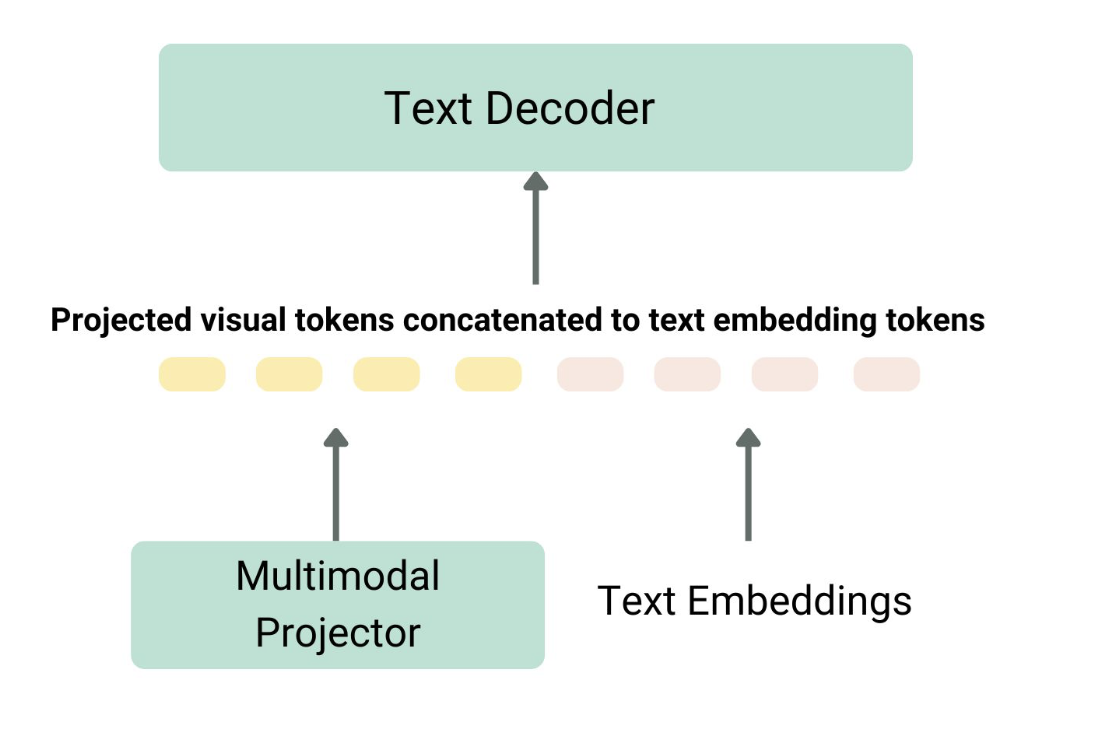
\includegraphics[width=0.5\linewidth]{figures/vlm}
    \caption{VLM 的架构（据 LLaVa \citep{liu2023visual}，图片来自 Huggingface）}
    \label{fig:vlm}
\end{figure}


\begin{figure}
    \centering
    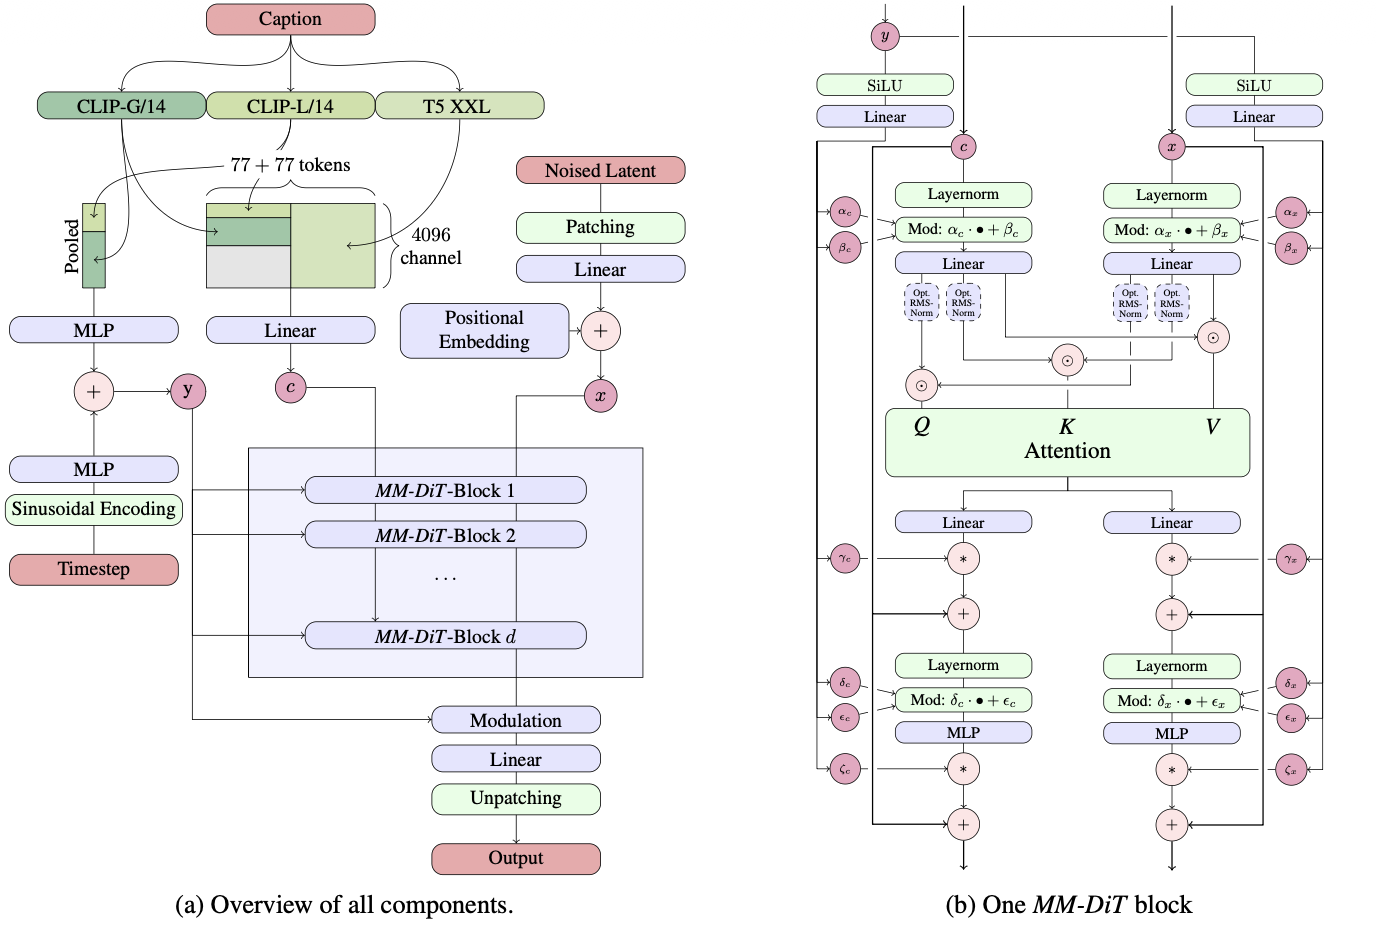
\includegraphics[width=0.95\linewidth]{figures/stable}
    \caption{Stable Diffusion 的架构 \citep{esser2024scaling}}
    \label{fig:stable}
\end{figure}

然后，人们需要一种架构来融合语言嵌入与图像嵌入，并生成语言。
总体而言，VLM 的架构由一个图像编码器（可以是 CNN，也可以是经过专门词元化的视觉 Transformer）和一个文本编码器构成，二者连接到嵌入投影器，把图像与文本表示对齐（通常是一个稠密神经网络），最后连接到文本解码器（一个 Transformer）。图~\ref{fig:vlm} 以 LLaVa 为例展示了这一架构 \citep{liu2023visual}。
视觉嵌入与文本嵌入之间的连接，由一个网络完成——它把视觉嵌入投影到另一种嵌入上，以便模型做统一推理。投影器网络通常是稠密神经网络（多层感知机，MLP）。

人们已开发出更精细的架构，最先进 VLM 的架构可能变得相当复杂，由多个 Transformer 模块组成。例如，图~\ref{fig:stable} 展示了生成式的 Stable Diffusion 架构 \citep{esser2024scaling,weng2021diffusion,yang2023diffusion}。

\subsection{学习算法}
既然已经看到 VLM 的任务与架构，现在来看模型所用的学习算法类型。
不同的编码器与投影器使 VLM 得以训练。训练算法应当对齐并融合来自视觉编码器与语言编码器的知识。这样 VLM 就能关联图像与文本信息，从而能分析查询、并基于两种模态给出答案。文献报告了训练 VLM 的多种不同方法。

OpenAI 的 CLIP \citep{radford2021learning}，全称{\em 对比语言—图像预训练}，使用对比学习。对比学习是自监督学习的一种形式，当数据集中没有标签时，它自行构造监督信号。其想法是在嵌入空间中把不相似的数据点推远、把相似的数据点拉近。对比学习最大化{\em 正样本}对（如同一图像的不同形式）表示的相似度，并最小化{\em 负样本}对（不同物体的图像）的相似度。%The VLM is trained on a dataset of image-text pairs. It maps the image and text embeddings from the encoders into a joint  embedding space to predict the correct pairings, it minimizes the distance between embeddings of matching pairs, and maximizes it for non-matching pairs. 

%Arch:
%- language encoder. Transformer
%- image encoder. First CNN, now ViTransformer

%Learning Algorithm:
%- constrastive. CLIP
另一种方法是使用掩码。这里 VLM 学习预测输入文本或图像中被随机遮蔽的部分，就像在语言模型训练中那样。模型学习在给定（未掩码）描述的情况下，重建图像中被隐藏的像素。一个例子是 FLAVA，即{\em 基础语言与视觉对齐}，它用视觉 Transformer 作图像编码器、用 Transformer 作语言编码器与多模态投影器 \citep{singh2022flava}。

%- masking. FLAVA
\begin{figure}
    \centering
    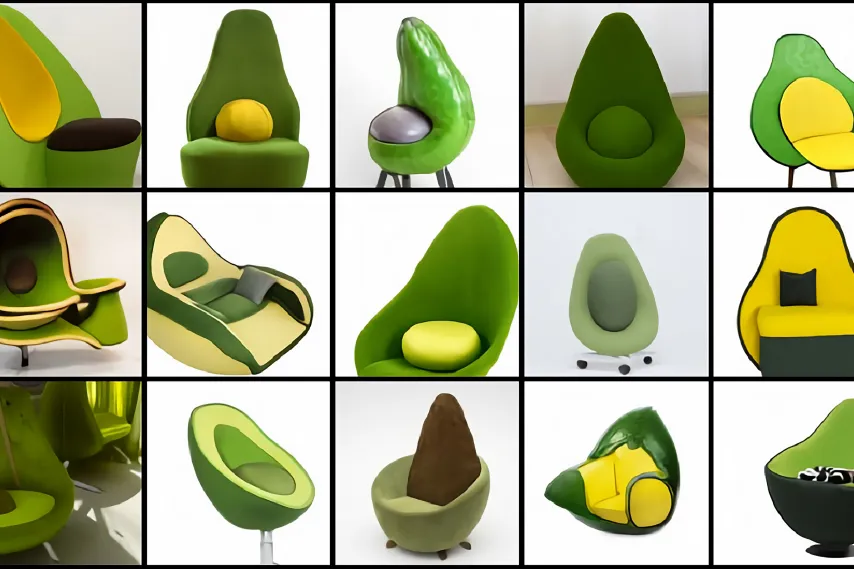
\includegraphics[width=\linewidth]{figures/dalle}
    \caption{DALL-E：鳄梨色扶手椅}
    \label{fig:dalle}
\end{figure}
VLM 也被以生成式方式使用，即根据文本提示生成图像。流行的文本到图像模型常用扩散模型 \citep{ho2022large,yang2023diffusion}。著名例子有 Google 的 Imagen \citep{baldridge2024imagen}、Midjourney、OpenAI 的 DALL-E \citep{betker2023improving} 以及 Stability AI 的 Stable Diffusion \citep{esser2024scaling}。DALL-E 2 使用以 CLIP 图像嵌入为条件的扩散模型。图~\ref{fig:dalle} 展示了 DALL-E 那组著名的超现实主义鳄梨扶手椅。

%- pretrained. LLAVA

%Contrastive: maps the image and text embeddings from both encoders into a joint or shared embedding space. The VLM is trained on datasets of image-text pairs and learns to minimize the distance between embeddings of matching pairs and maximize it for nonmatching pairs. CLIP

%Masked: in masked image modeling, VLMs learn to reconstruct the hidden pixels in an image given an unmasked caption. The multimodal encoder applies a cross-attention mechanism to integrate textual and visual information. FLAVA’s training encompasses masked modeling along with contrastive learning.

%Generative: 
%learning to generate new data. Text-to-image generation produces images from the input text, while image-to-text generation produces text—such as captions, image descriptions or summaries—from an input image. Examples of popular text-to-image models include diffusion models, such as Google’s Imagen, Midjourney, OpenAI’s DALL-E (beginning with DALL-E 2) and Stability AI’s Stable Diffusion.

%Pretrained:
从头预训练视觉语言模型代价高昂，而且既然 VLM 由语言模型与视觉模型组成，我们可以尝试看看能否用一或两个已经预训练好的现有模型拼出一个 VLM。
既可以用一个预训练好的 LLM，也可以用一个预训练好的视觉编码器，再加一个映射网络，把视觉嵌入投影到语言模型的文本输入空间中。
一个例子是 LLaVA，全称{\em 大语言与视觉助手}。LLaVA 使用 Vicuna 语言解码器与 CLIP ViT 视觉编码器，二者输出通过一个线性投影器融合到同一维度空间中 \citep{liu2023visual}。

人们已开发出许多视觉语言模型。VLM 往往在基准任务上表现良好，且常被用于智能体的决策。
VLM 已流行到这种程度：当前许多开放与商用 LLM 都是 VLM：DeepSeek-VL2、Gemini 2.0 Flash、GPT-4o、Llama 3.2、NVLM、Qwen 2.5-VL。



\begin{figure}
    \centering
    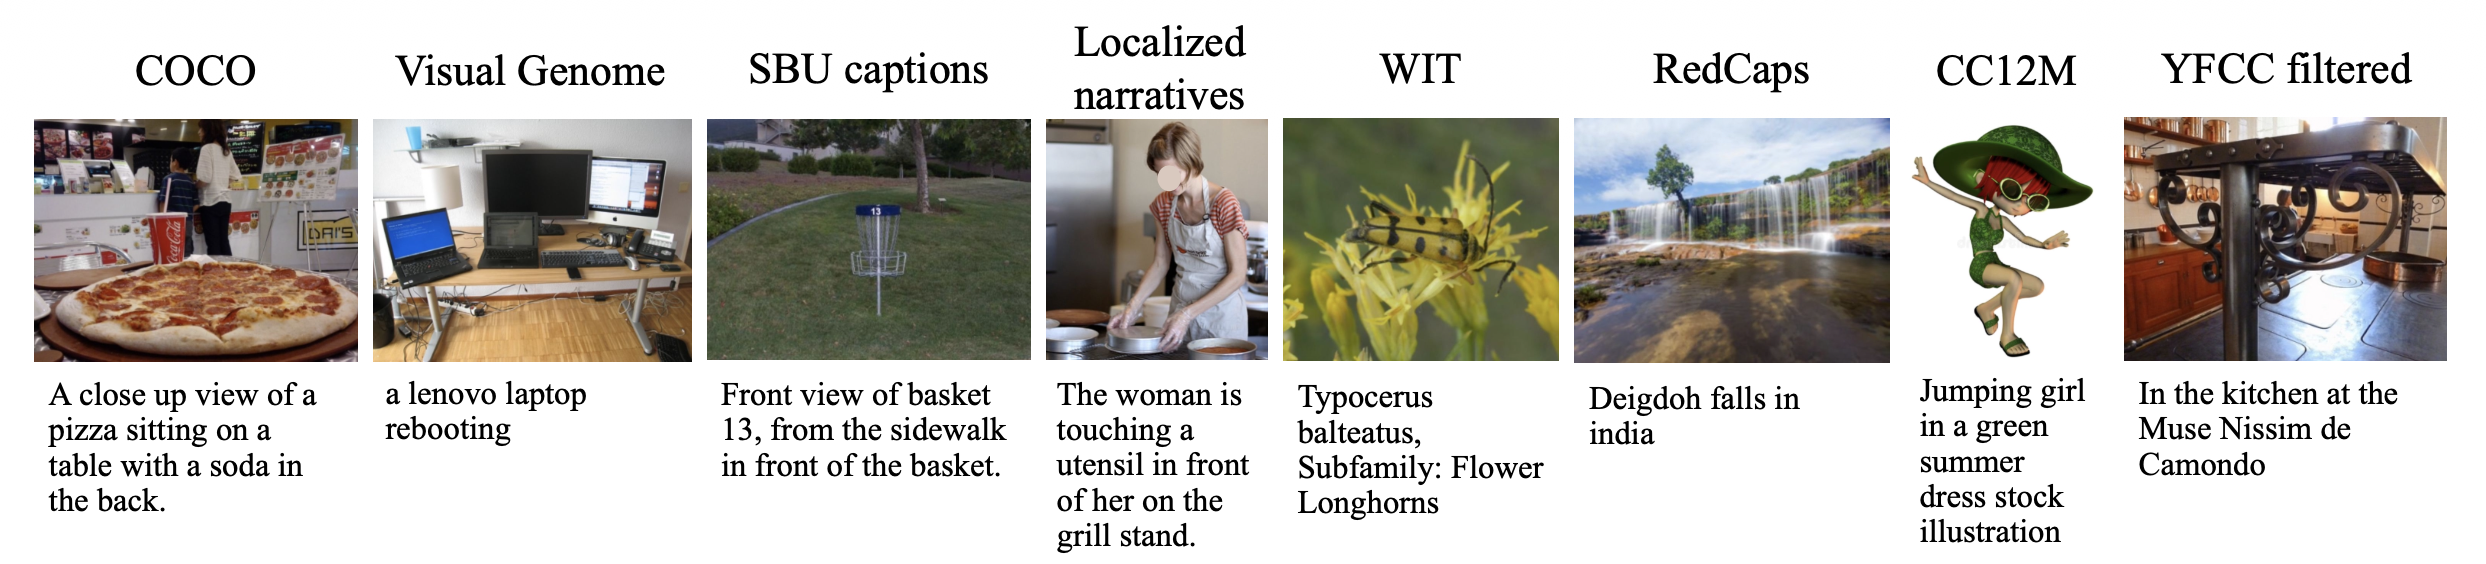
\includegraphics[width=\linewidth]{figures/flava}
    \caption{FLAVA 预训练图像—文本数据集示例 \citep{singh2022flava}}
    \label{fig:flava}
\end{figure}

\subsection{结果}
我们来看看文献所报告的例子中，VLM 在图像描述与图像生成方面表现如何。

视觉语言模型已产出富有想象力与启发性的成果，从视觉问答、目标检测、图像描述到文本到图像生成，不一而足。图~\ref{fig:flava} 展示了 FLAVA 所用测试数据集的一个例子。DALL-E 2 的继任者 DALL-E 3 专注于在高描述性生成图像描述上训练，取得了更令人瞩目的成果 \citep{betker2023improving}。DALL-E 3 的部分提示词遵循图像生成能力见图~\ref{fig:dalle3}。图~\ref{fig:stablediff} 展示了 Stable Diffusion 的例子（基于整流流扩散模型）。


\begin{figure}
    \centering
    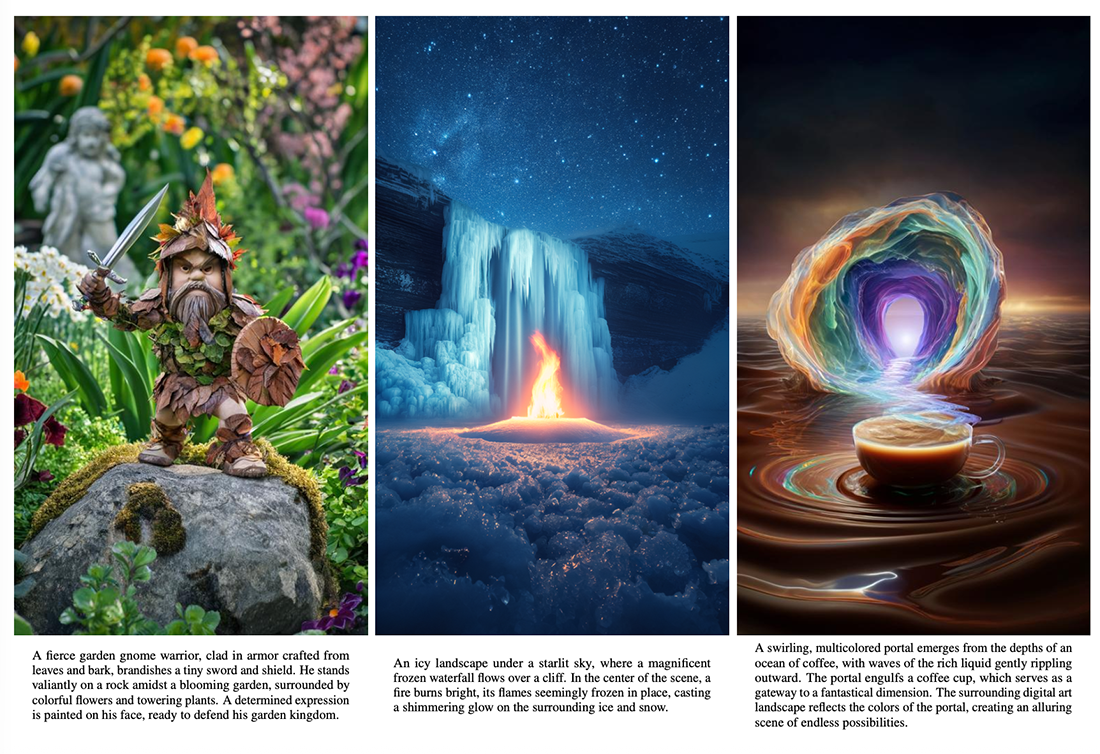
\includegraphics[width=\linewidth]{figures/dalle3}
    \caption{来自 DALL-E 3 的遵循提示词的文本到图像示例 \citep{betker2023improving}}
    \label{fig:dalle3}
\end{figure}


\begin{figure}
    \centering
    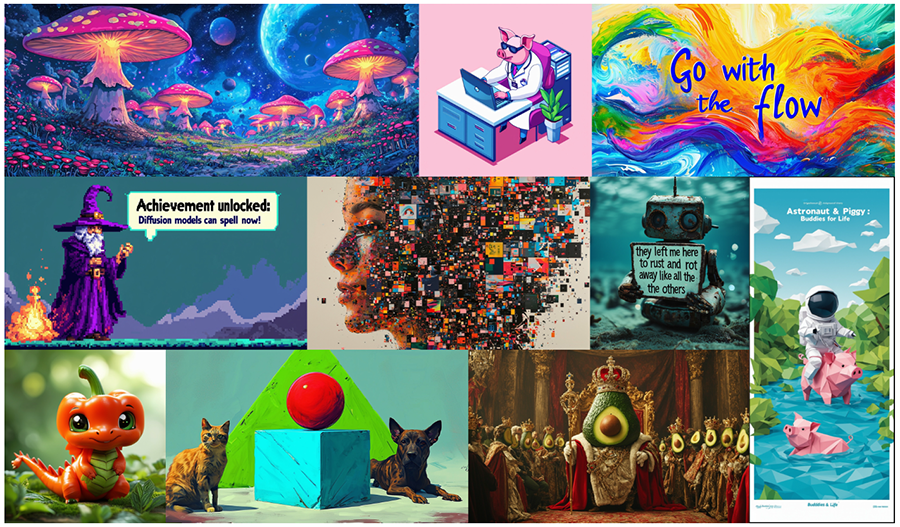
\includegraphics[width=\linewidth]{figures/stablediff}
    \caption{Stable Diffusion 示例 \citep{esser2024scaling}}
    \label{fig:stablediff}
\end{figure}


\begin{figure}
    \centering
    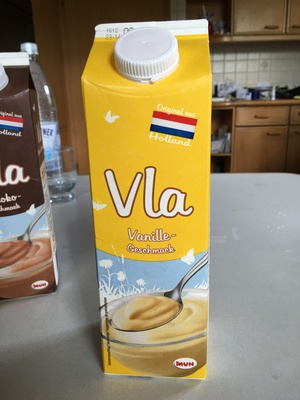
\includegraphics[width=0.4\linewidth]{figures/vla.jpg}\ 
        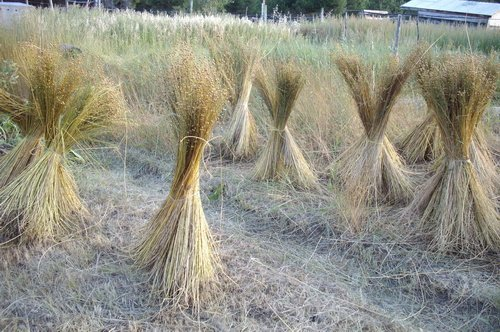
\includegraphics[width=0.4\linewidth]{figures/vlas.jpg}
    \caption{VLA 在不同语言中有不同含义。Vlas 也是如此。（其中一张图暗示了这是哪种语言）}
    \label{fig:vla}
\end{figure}
\section{决策与视觉—语言—动作模型}\label{sec:vla}

%\paragraph{Vision-Language-Action Models}
要行动，智能体就必须做决策；而要做决策，就必须权衡不同选项。%The previous chapter showed methods for external prompt optimizers to search the tree of possibilities and in-context learning. We also saw in Section~\ref{sec:decisions} that the transformer architecture can  be pretrained to facilitate decision making, and reinforcement learning. %At the end of this chapter we will discuss this approach in more depth. %\todo{AGAIN??? We did that in 6.2.4. Hmm. In this chapter the DT story is longer. Where does it fit best? It does fit in 6.2.4. But also in 7.4. Gewoon zeggen dat we het al eens eerder gezien hebben?}
正如我们将在本节看到的，%in addition to training transformers on sequences of tokens that represent language and pixels, 
我们可以在由状态、动作与奖励组成的回合（episode）$\{(s,a,r)\}$ 上训练 Transformer（另见第~\ref{sec:decisions} 节）。
%
这些模型在语言、视觉与机器人动作的序列上训练。视觉—语言—动作模型（VLA，图~\ref{fig:vla}）被训练来输出机器人 API 命令——这是一类特殊的语言：用于操控机器人运动的命令语言。%Various pretraining and interacting on large datasources has yielded impressive generalization by VLAs \citep{black2024pi_0,team2023gemini}.

%After vision, the next step is to add actions to the model. Models that are trained on vision, language and actions are called vision-language-action models, or VLA (see Figure~\ref{fig:vla}). 
VLA 的任务是理解一个视觉场景，并在给定文本命令时，指示机械臂根据模型通过摄像头看到的情况执行恰当的动作。
这些模型已展示了机器人泛化到未见情境、成功完成任务的惊人成果。

\begin{figure}
    \centering
    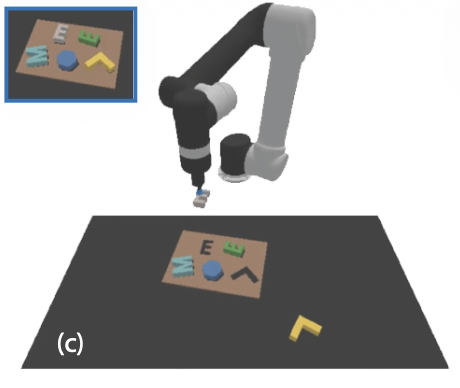
\includegraphics[width=0.5\linewidth]{figures/cliport1}
    \caption{来自 CLIPort 的例子：{\em 把灰色的字母 E 放进左边的 E 形孔} \citep{shridhar2022cliport}}
    \label{fig:cliport1}
\end{figure}

\subsection{任务}
VLA 的主要任务是在现实世界中执行指令，并且以一种通用的方式、在不断变化的环境中做到这一点。当一个机器人操作模型被训练去捡一叠红色铅笔，而任务变成捡蓝色铅笔时，理想情况是模型能泛化，我们不必重新组装一套涉及蓝色铅笔的训练集、从头再训练一遍。我们还希望模型能识别物体，并识别物体何时朝向不同、发生了移动，或光照发生变化。模型应当知道如何用机械臂操作物体，以及如何执行不同的动作。例子见图~\ref{fig:cliport1}，取自 CLIPort 论文 \citep{shridhar2022cliport}。


\begin{figure}
    \centering
    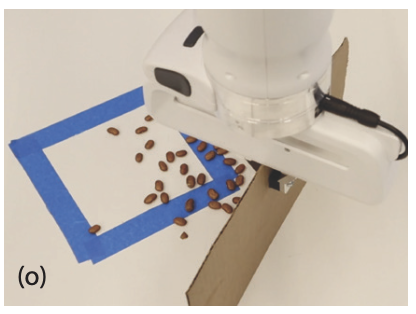
\includegraphics[width=0.5\linewidth]{figures/cliport2}
    \caption{来自 CLIPort 的另一个例子：{\em 把豆子扫进蓝色区域} \citep{shridhar2020alfworld}}
    \label{fig:cliport2}
\end{figure}

VLA 最困难的任务，是把这些场景、物体与动作组合成训练中所见内容的复杂组合操作，并泛化到未见过的组合。尤其是穿越复杂、多变（甚至可能是户外）环境的长时间跨度导航，是一项复杂挑战 \citep{shridhar2022cliport}。

在真实的人机交互情境中，
收集额外演示往往不可行。
要执行图~\ref{fig:cliport2} 这类高层任务，VLA 必须能够识别物体、它们的姿态，以及实例分割。模型还必须能理解语言，并把语言的意义与视觉物体的意义、以及与机器人动作的意义关联起来。

正如我们将看到的，语言为指定目标和在不同任务间
迁移语义概念提供了一个直观接口。此外，VLM 方面的工作已经展示了如何在语义上连接不同种类的嵌入。

%Describe
%significantly improved generalization to novel objects, the ability
%to interpret commands not present in the robot training data (such as placing an object onto a particular
%number or icon), and the ability to perform rudimentary reasoning in response to user commands (such
%as picking up the smallest or largest object, or the one closest to another object). We further show that
%incorporating chain of thought reasoning allows RT-2 to perform multi-stage semantic reasoning, for
%example figuring out which object to pick up for use as an improvised hammer (a rock), or which type
%of drink is best suited for someone who is tired (an energy drink).

%long-horizon navigation through complex, outdoor envi-
%ronments from natural language instructions

%capable of solving a variety of language-specified tabletop tasks from packing
%unseen objects to folding cloths, all without any explicit representations of object
%poses, instance segmentations, memory, symbolic states, or syntactic structures.
%Experiments in simulated and real-world settings show that our approach is data
%efficient in few-shot settings and generalizes effectively to seen and unseen se-
%mantic concepts. We even learn one multi-task policy for 10 simulated and 9
%real-world tasks that is better or comparable to single-task policies.

%Mobility VLA in a 836m2 real world environment and
%show that Mobility VLA has a high end-to-end success rates on previously unsolved
%multimodal instructions such as "Where should I return this?" while holding a plastic
%bin.


%Generalization: Give textual instruction to robot to move in visual scene. 

\subsection{架构}
既然已经看到任务与挑战，现在来看可能的模型架构。同样，它们也可能变得相当复杂。
Transformer 架构很擅长学习序列数据中的模式，自然语言上的结果已经说明了这一点。直观上，这表明 Transformer 也可能很适合为顺序决策问题建模——这类问题常在机器人动作的强化学习中求解，如我们在第~\ref{sec:sdp} 节所讨论的（并在第~\ref{sec:icrl} 节深入展开）。这类问题由一个状态构成，从该状态出发的动作使系统进入新状态，新状态又有动作，如此往复。Transformer 架构很适合为这些问题建模。

早期关于决策 Transformer（DT）的工作 \citep{chen2021decision,janner2021offline} 表明，在离线（静态）强化学习问题上，GPT 架构确实能学到最优策略。决策预训练 Transformer（DPT）\citet{lee2023supervised,wang2024transformers} 则表明，基础 Transformer 架构可以在决策轨迹上预训练与微调。第~\ref{sec:decisions} 节会进一步讨论决策轨迹。

继 CLIPort \citep{shridhar2022cliport,shridhar2020alfworld} 的开创性工作之后，VLA 常建立在 VLM 之上，其中机器人命令被当作普通语言词元使用。让我们仔细看几个有代表性的模型。


Mobility VLA \citep{chiang2024mobility} 的目标是导航。这个 VLA 由长上下文 VLM 与拓扑图结合而成，如图~\ref{fig:mobility} 所示。
\begin{figure}
    \centering
    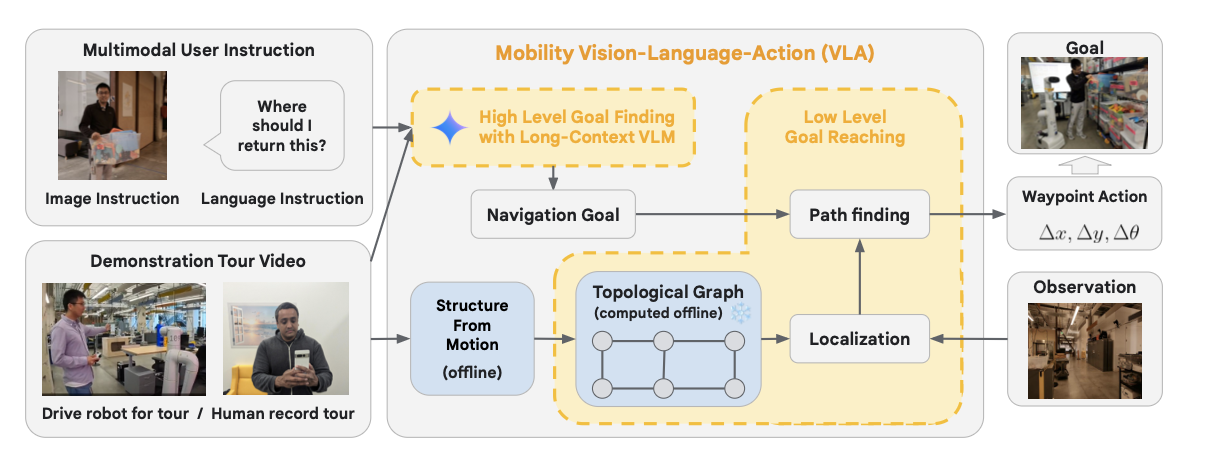
\includegraphics[width=0.95\linewidth]{figures/mobility}
    \caption{Mobility VLA 架构：长上下文 VLM 与拓扑图 \citep{chiang2024mobility}}
    \label{fig:mobility}
\end{figure}
Mobility VLA 用于一类称为{\em 带演示巡视的多模态指令导航}（MINT）的导航任务。在这个数据集中，通过一段预先录制的演示
视频提供环境先验。该模型由一个两级 VLA 构成，把长上下文 VLM 的环境
理解与常识推理，同基于拓扑图的
低层导航策略结合起来。高层策略由长上下文 VLM 结合，在演示视频中找到目标帧来构成
用户指令。随后，低层策略从该目标帧出发，遍历一张拓扑图，在每个时间步生成机器人动作指令。

LM-Nav \citep{shah2023lm} 使用另一种基于现有模型的架构。它接收来自目标环境的一组原始观测
以及自由形式的文本指令。由此，它用三个预训练模型推导出一个行动计划：一个语言模型（LLM）用于提取地标、一个视觉—语言模型（VLM）
用于落地，以及一个视觉导航模型（VNM）用于执行（与前面讨论的拓扑图不无相似）。这些模型合起来
使 LM-Nav 能在不进行任何微调的情况下，从视觉观测中遵循文本
指令。该方法的说明见图~\ref{fig:lmnav}。
\begin{figure}
    \centering
    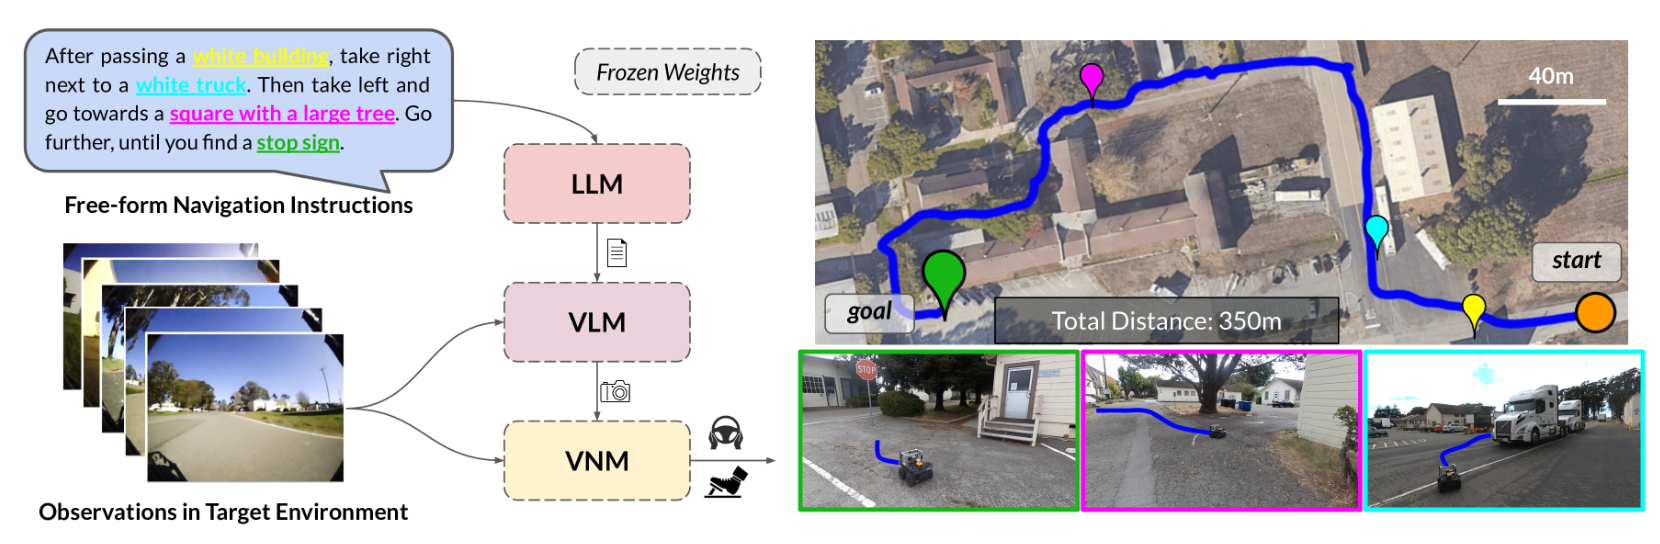
\includegraphics[width=0.95\linewidth]{figures/lmnav}
    \caption{LM-Nav 的三模型架构 \citep{shah2023lm}}
    \label{fig:lmnav}
\end{figure}


Google 的 RT-2 \citep{brohan2023rt} 采用了不同方法。RT-2 的思路是利用网络世界的知识来指导机器人控制：机器人应当通过看视频来学会如何行动。一个标准视觉语言模型同时在文本机器人轨迹数据和
互联网规模的视觉—语言任务（如视觉问答）上微调。机器人动作被表示为普通文本词元，并直接
并入训练集，方式与自然语言词元相同，如图~\ref{fig:rt2} 所示。
\begin{figure}
    \centering
    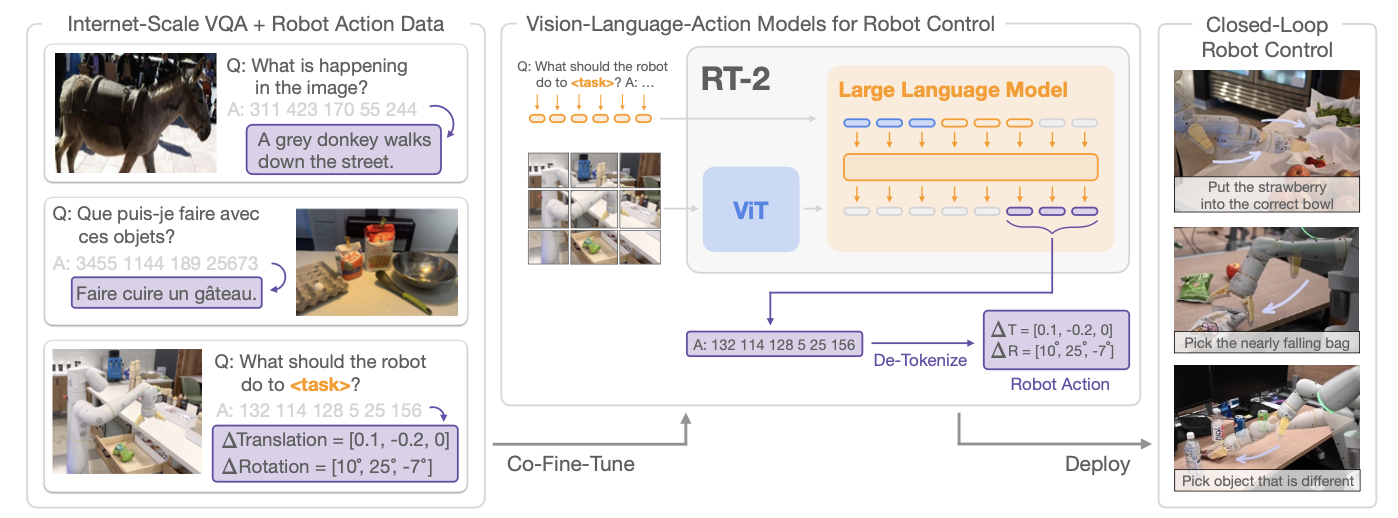
\includegraphics[width=0.95\linewidth]{figures/rt2}
    \caption{RT-2 架构：用机器人动作作为文本词元训练的 VLM \citep{brohan2023rt}}
    \label{fig:rt2}
\end{figure}
Magma \citep{yang2025magma} 采用了类似途径。Magma 在从图像、视频到机器人数据的异构数据集上预训练。不过，在 Magma 中，图像里可动作的视觉物体
用特殊词元（Set-of-Mark）标注，以落实动作。类似地，物体的运动（如人手或
机械臂的轨迹）用 Trace-of-Mark 
标注，以便进行动作规划。说明见图~\ref{fig:magma}。
\begin{figure}
    \centering
    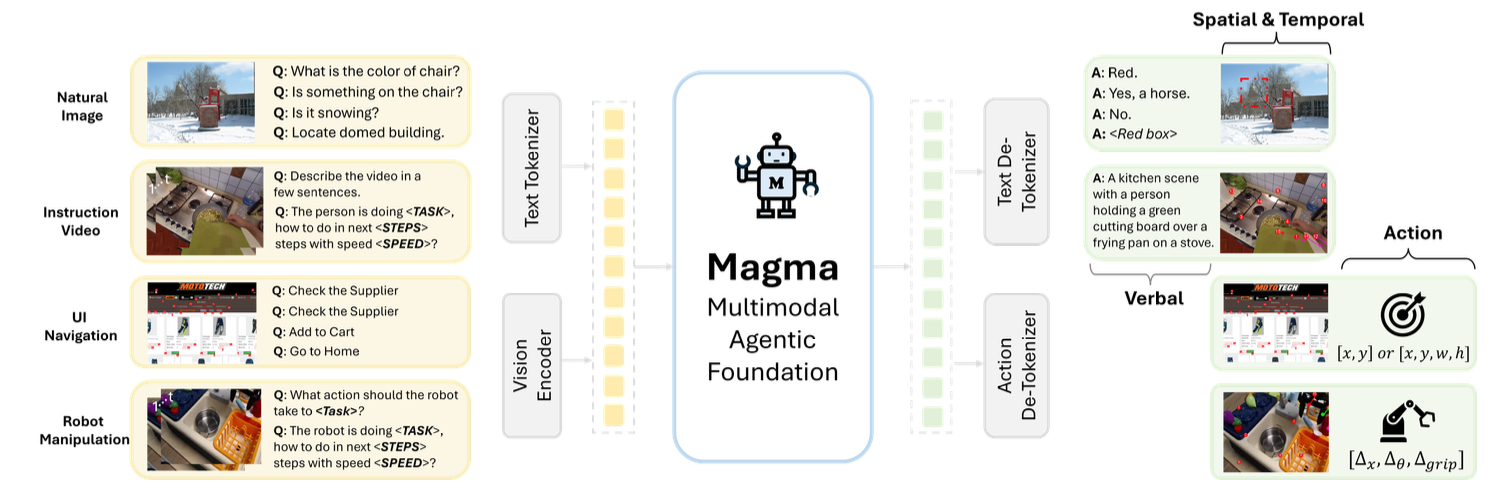
\includegraphics[width=0.95\linewidth]{figures/magma}
    \caption{Magma 预训练流水线 \citep{yang2025magma}}
    \label{fig:magma}
\end{figure}

最后，一个名为 $\pi_0$ 的 VLA \citep{black2024pi_0} 强调强化学习途径：它使用一个预训练的后期融合视觉—语言模型，以及一个涵盖多种
操作任务的多样化跨本体数据集。该模型受 Transfusion 方法启发 \citep{zhou2024transfusion}。它为适配机器人控制，加入了一个单独的
动作专家，通过流匹配产生动作，以获得流畅的操作技能。所得模型
既可以直接用于根据提示词执行任务，也可以在更高质量的数据上进一步微调，以完成复杂的多阶段
任务，例如叠多件衣物或组装一个盒子（见图~\ref{fig:pizero}）。
\begin{figure}
    \centering
    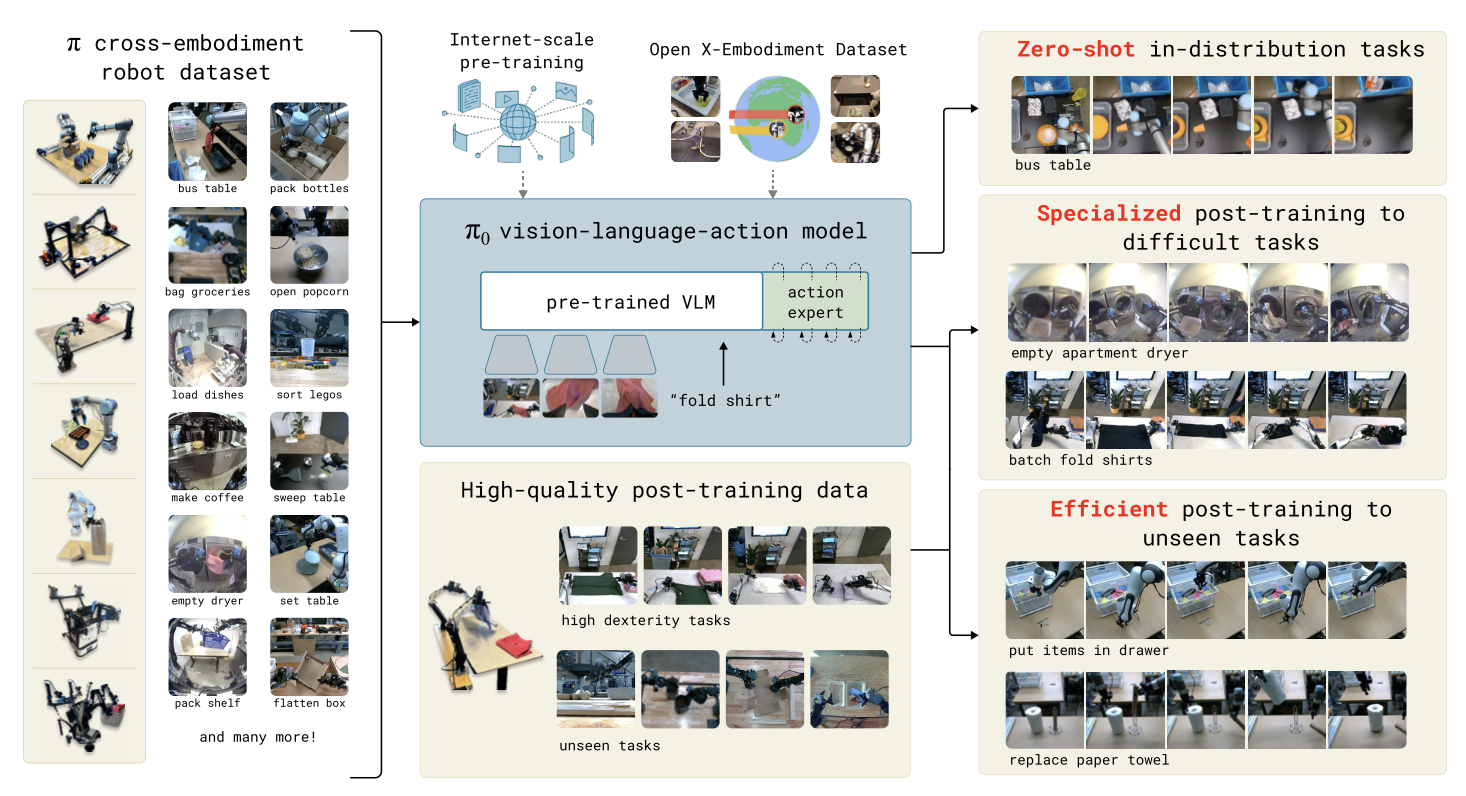
\includegraphics[width=0.95\linewidth]{figures/pizero}
    \caption{$\pi_0$ 的架构。该模型基于 VLM，并用跨本体数据集增强 \citep{black2024pi_0}}
    \label{fig:pizero}
\end{figure}








\subsection{学习算法}
大多数 VLA 的模型架构基于 VLM，有些还用导航地图数据增强。机器人动作命令通常被编码为普通文本命令。同样，在预训练与微调中使用的是典型的 LLM 自监督学习算法，与 VLM 和决策 Transformer 类似。有时会使用现有预训练模型，以降低训练开销。


\subsection{结果}
已有
各种 VLA 模型被创造出来，取得了惊人的零样本结果，把行为泛化到未见情境。
\citet{chiang2024mobility,brohan2023rt,yang2025magma} 是
面向机器人动作的 VLA 模型例子，能完成导航、桌面操作乃至叠衣服等复杂任务 \citep{black2024pi_0}。


VLA 已展示出惊人而富有想象力的成果，机器人能在不重新训练的情况下于推理时泛化。VLA 的综述可参见
\citep{ma2024survey}。

这些成果最好通过看视频来体会。
对 $\pi_0$，有视频
可看。\footnote{\url{https://www.physicalintelligence.company/blog/pi0}} 
对 RT-2，也有视频
可看。\footnote{\url{https://robotics-transformer2.github.io}} 




%Embodied problems require an agent to understand  semantic aspects of the world: the topology, the repertoire of skills available, how these skills influence the world, and how changes to the world map back to language. When the model is prompted to move a cup on a table, it helps when the LLM knows if the agent has limbs that allow it to move objects, and whether it is in a room where a table and a cup are present.

%By leveraging environment feedback, LLMs are able to form an inner monologue that allows them to more richly process and plan in robotic control scenarios.
%
%Language models contain a large amount of information about the real world \citep{ahn2022can}. In theory, this may allow the model to exhibit realistic reasoning about robotic behavior. %However, the models do not have knowledge about particular embodied aspects of a particular robot. 
%If we could compare a list of intermediate reasoning steps with a list of possible movements of the robot in its environment, then we could prevent the model from suggesting impossible joint movements and actions, and prevent errors or accidents. 
%Such an approach has been tried in the Say Can paper
%\citep{ahn2022can}. Say Can learns a value function \citep{kaelbling1996reinforcement} of the behavior of a robot in an environment using  temporal difference reinforcement learning \citep{sutton1988learning}. This value function is then  combined with prompt-based reasoning by the language model, to constrain it from suggesting impossible or harmful actions. 
%
% {\bf What does SayCan say? Is it like Scratchpad?}
% Note that Scratchpad was trained by supervised learning on a
% pre-existing dataset. The goal of Say-Can is to create a  robotic
% affordance model, by using reinforcement to learn a value
% function. A separate language model is used for  prompt learning, to
% incorporate the learned value function in the prompts.  
%
%The goal of Say Can is to ground the language model in robotic
%affordances. %  The affordance model is learned interactively by reinforcement
% learning, and then applied using prompt-based learning by
% the LLM. 
% The robot can act as the language model’s hands and eyes, while
% the language model has high-level semantic knowledge about the
% task.  The LLM (Say) provides a task-grounding to find the actions to
% achieve the high-level goal. The learned affordance function (Can)
% provides a world-grounding to allow what is possible. 
% Reinforcement
% learning learns language-conditioned value functions that provide affordances of what
% is possible in the world.
%Say Can is evaluated  on 101
%real-world robotic tasks, such as how to solve tasks in a kitchen environment (see Figure~\ref{fig:saycan}).


%\begin{figure}
%  \begin{center}
%    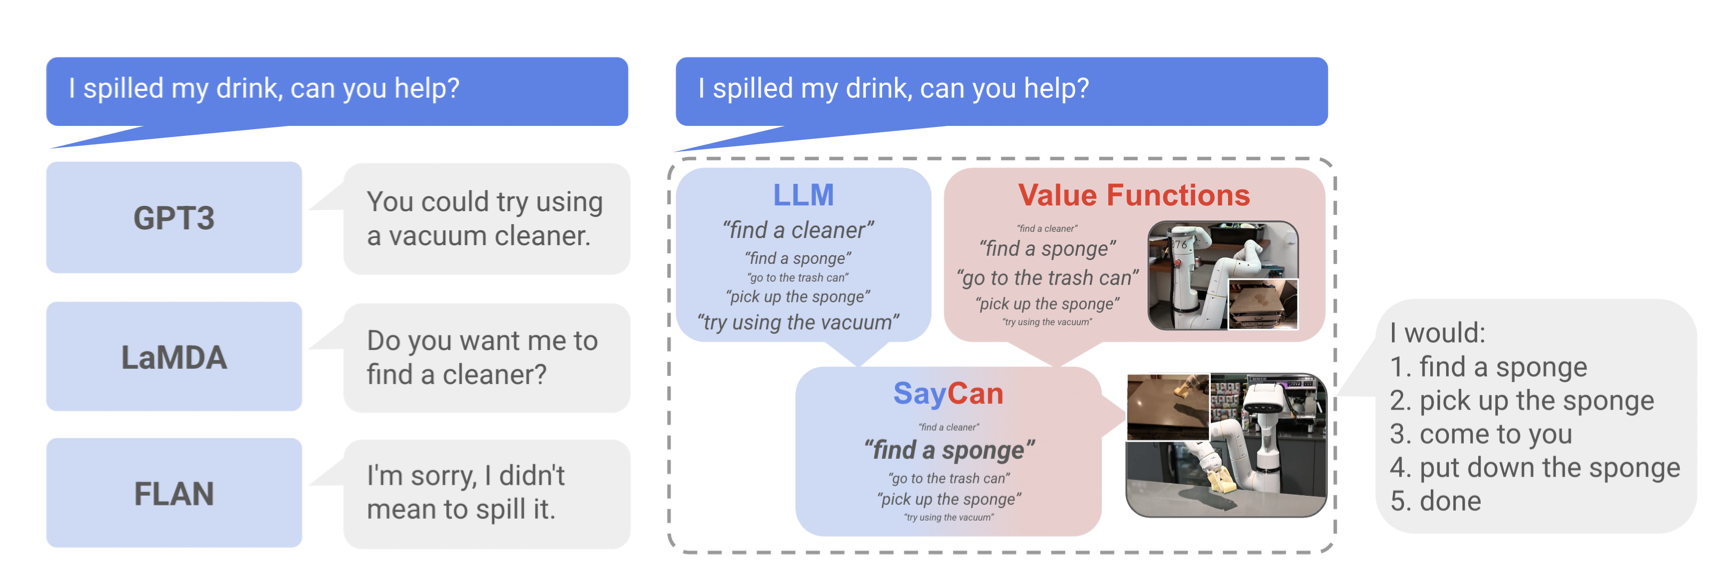
\includegraphics[width=14cm]{figures/saycan}
%    \caption{Say Can compared to other language models \citep{ahn2022can}}\label{fig:saycan}
%  \end{center}
%\end{figure}

%\citet{liu2023llm} combine an LLM with  a
%combination of teleoperation and Dynamic Movement Primitives is
%employed for action correction.

\section{世界模型、物理与规划}\label{sec:world}

%\paragraph{World Models}
对 VLM 而言，一幅图像由像素构成，没有更深层的内在意义。然而，与世界交互的智能体需要关于那个世界的物理属性的知识。%As we discuss in Section~\ref{sec:world}, 
这些模型需要理解什么在物理上是可能的，这样智能体才不会穿墙而过——正如它们在电子游戏中偶尔还会做的那样。%
%As LLMs incorporate more data modalities, they acquire more world knowledge. The multi-modal models that we discuss in this chapter increasingly fit the requirements to act as a source of knowledge about the world in which agentic LLMs operate. 

%Agents receive feedback when they act in the world. A world model requires a mechanism to learn from this feedback. Reinforcement learning, the type of machine learning that learns actions from feedback, offers such a mechanism.
%World models have been researched for quite some time in machine learning. In model-based reinforcement learning in particular, world models play a central role \citep{sutton1991dyna,moerland2023model,hafner2020mastering,plaat2020deep}.
%, and the training of world models has been studied. 
%These world models are trained on feedback from interaction of the agent with the world. %A model is built that  is then used to improve further interactions by the agent with that world. 
%Reinforcement learning provides a useful framework for training world models, and reinforcement learning methods are used extensively to build agentic world models with a form of understanding of physics. 

%\paragraph{Decision Transformer}
%\todo{Hmm. Is dit nu ge-delete?}


%The new modalities introduce new names: vision-language models are called VLMs, models with robotic actions are called VLAs, and models that aim to understand the physics of the world  are called {\em world models}. Note that from now on we may use the term {\em LLM} to include these new, richer models. 
%We will now start with the first modality that is added to LLMs: vision.

%In this section we will introduce world models. 
世界模型帮助智能体理解世界，使它们能在物理世界中有效地行动，做出有意义的动作。最初，LLM 是语言模型。我们可以用自然语言与它们交谈，而它们必然包含某些世界知识，但并未经过专门训练以对世间万象有广而深的理解。一些研究者认为，要让智能体大语言模型真正成功、要让 LLM 达到很高的通用智能水平，就应当加强世界模型研究 \citep{sutton2022alberta,matsuo2022deep,lecun2022path,klindt2026does}。

%Vision language models add an important skill, allowing visual understanding by the agent, and VLAs add certain types of actions to the model, mostly in the realm of robotic arm movement. Research into world models extends this trend, and specifically focuses on adding knowledge to the reasoning model that will allow our agents to function well in the physical world. If this sounds as if the field is in motion, it is. World models are an active field of research, and we will discuss as much as we can of the state of the art. 


%LLMs are more and more regarded as world models from which an agent can sample to learn to improve a policy of good actions. Therefore, in this section we will review recent world model research. 

在世界中行动的智能体与机器人需要对世界的物理规律有初步理解。
训练 LLM 的一大挑战，是把它对物理世界及可能的机器人动作的理解落地到现实。
一种做法是从动作反馈中学习一个世界的智能体式模型（环境）。

%From VLM, to VLA, the step to training a World model seems a small next step. 
{\em 世界模型}这一术语在 AI 的其他语境中也用过。最著名的是指基于模型的强化学习中的{\em 模型} \citep{ha2018world,moerland2023model,sutton1991dyna}（见下一节）。%The meaning of the term {\em world} in reinforcement learning is the same as in agentic LLM: 
这个模型包含着环境的部分知识的本地副本，其基础是它与环境发生过的交互，用于改进动作策略。
世界模型包含着世界的一种高效、压缩、学到的表示 \citep{hafner2018learning,plaat2020deep}。世界模型的表示常被称为抽象的或{\em 潜}表示，以区别于环境中真实世界的常规表示。
世界模型常被训练来包含关于物理与某些空间属性的知识，这些知识限制了智能体的动作。% (to prevent it from attempting to walk through walls, for example).  
世界模型的确切内容取决于智能体所处的领域。




请注意，仅仅几章之内，我们就从理解语言走到了理解世界。大型{\em 语言}模型的目标，是从文本的统计模式中理解自然语言的某些语义，用于问答与翻译。而{\em 世界}模型的目标，是理解物理定律中的因果关系，用来为我们的智能体模拟未来的世界状态。从 LLM 走到智能体大语言模型，需要相当多的新技术。


我们先来看看世界模型目前在智能体大语言模型中是如何使用的。

\subsection{任务}
世界模型应当封装关于世界的知识，使智能体能执行有意义的动作。这些动作应当扎根于物理世界。例如，模型应当理解它正在指挥的机械臂的关节限制；一个导航智能体应当理解一些物理规律，比如重力、距离的概念，以及墙是实体；一个金融智能体应当理解银行余额为负的后果。这些往往是人类视为理所当然的信息，因此当一个智能体连它所处世界的这类基本事实都无法理解时，我们会感到意外。只在像素上训练过的 VLM，可能会错过某种纹理的语义含义——它究竟是衣物、烟雾，还是一堵墙。

标准的预训练 LLM 已经包含一些有用的世界知识。它们通过基于人类反馈的强化学习（RLHF）学会可接受的文本行为，通过可验证奖励强化学习（RLVR）学会可接受的数学与编程行为。一些早期方法把 LLM 当作世界模型使用，不做任何微调。
了解世界物理规律的一种自然方式是通过交互：智能体可以通过强化学习式的奖励函数学到可接受的物理行为。

%Reasoning via Planning (RAP) \citep{hao2023reasoning}, for example, follows a reinforcement learning design where the LLM is used for the separate functions of an MDP (action selection function, transition function, reward function), with a Monte Carlo Tree Search  planner (MCTS)~\citep{browne2012survey}. RAP achieves good results in blocksworld and GSM8K, using GPT and LLaMa LLMs in a pure ICRL setup, with MCTS. 

%Later approaches pretrain and finetune LLMs specifically as world model.
基于模型的强化学习中，世界模型的目标是通过用世界{\em 模型}做规划、而不是从{\em 真实}世界中采样，来提高从交互中学习的样本效率。当与世界的交互比执行一次模拟更昂贵时，这一点尤其有用——在智能体大语言模型中往往正是如此。在我们将讨论的这些方法中，LLM 世界模型使用来自基于模型的强化学习的方法（见第~\ref{sec:mbrl} 节）。目前，LLM 中的世界模型方法相当多样。为了说明世界模型在 LLM 中用于哪些任务，我们讨论三个例子：WorldGPT、WebDreamer 与 WorldCoder。

\paragraph{WorldGPT}
WorldGPT \citep{ge2024worldgpt} 的目标是解决视觉问答与具身规划任务，包括音视频问答。WorldGPT 从视频中学到一个世界 VLM。
它使用一个带外部知识库和长期记忆的潜空间 VLM。

\paragraph{WebDreamer}
WebDreamer \citep{gu2024your} 的目标是提高 Web 交互任务（如电子商务）的学习效率。WebDreamer 让 Web 智能体能在执行前先模拟动作，从而更快、样本效率更高（不必在真实网络上行动来收集经验）。WebDreamer 是 Web 世界中的一种基于模型的强化学习方法。（该名字源自{\em Dreamer}——一系列有影响力的基于模型的强化学习潜动力学模型~\citep{hafner2018learning,hafner2019dream,hafner2023mastering}。）典型任务是在电子商务网站上找商品。它通过从大模型训练出小模型来做到这一点，从而实现高效模拟。

%Be able to use LLM to simulate. Enable Model-based Planning for Web Agents before committing to real action. How can we build effective world models for the Internet? Unlike traditional world models in RL focusing on improving data efficiency in the agent learning process, LLM-based world models emphasize decision-making over simulation fidelity, leveraging broad world knowledge for planning. 

\begin{figure}
  \centering
    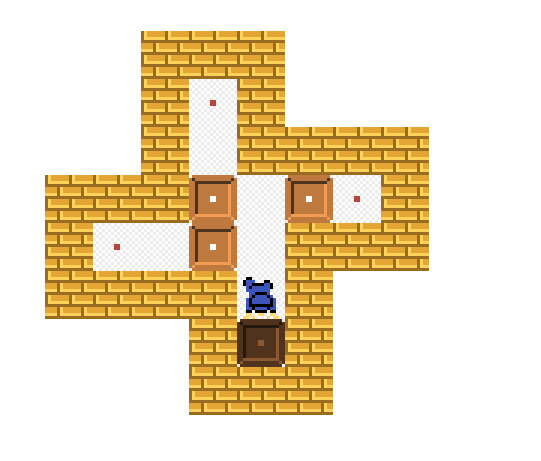
\includegraphics[width=7cm]{figures/sokoban}
    \caption{WorldCoder 用的推箱子~\citep{tang2024worldcoder}}\label{fig:sokoban}
\end{figure}

\begin{figure}
  \centering
    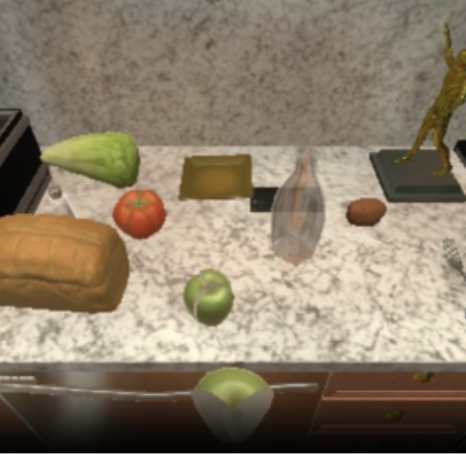
\includegraphics[width=6cm]{figures/alfworld}
    \caption{WorldCoder 用的 AlfWorld \citep{tang2024worldcoder}}\label{fig:alfworld}
\end{figure}

\paragraph{WorldCoder}
WorldCoder \citep{tang2024worldcoder} 的目标也是提高样本效率，但方法不同。%Its goal is also to improve sample efficiency, but i
WorldCoder 以可解释的 Python 代码生成动力学模型（转移函数与奖励函数），然后把它用于标准的基于模型的强化学习设计中。生成的 Python 代码执行起来比 LLM 推理更高效。WorldCoder 被用于网格任务（推箱子，见图~\ref{fig:sokoban}）与家务任务规划（AlfWorld，见图~\ref{fig:alfworld}）。


\subsection{架构}
世界模型的目的是给观测赋予语义——动作会产生后果——而这是 LLM 与 VLM 可能难以做到的。一个像素何时属于可以行走的地面（限制 $y$ 方向移动），何时又属于阻挡你的墙的一部分（限制 $x$ 方向移动）？奖励函数提供反馈信息，说明哪些动作好、哪些不好。因此，世界模型架构常用强化学习设定，在其中通过反馈奖励训练动作策略。我们可以把世界模型看作内部带一个策略学习器的 VLM。

WorldGPT、WebDreamer 与 WorldCoder 为各自的世界模型使用了不同架构，下面我们详细讨论。

\begin{comment}
\paragraph{WorldGPT Summary}
\begin{itemize}
    \item Goal: Understand World Dynamics. WorldGPT is capable of synthesizing dynamic scenes that change according to complex interactions.
    \item Data: Analyze internet videos.
    \item Architecture: WorldGPT is World Simulator. Help synthesize multimodal instruction instances. Built on MLLM. Specialized/long-term tasks: cognitive architecture (memory, knowledge retrieval, context reflection). Composed of 3 modules: Multimodal encoders, LLM to predict state transisiotns, multimodal decoder. Architecture diagram. Cognitive architecture: Knowledge, Memory, Context Reflector (built on Q-former \citep{li2023blip}).
    \item Learning Algo: Built on pretrained MLLM Vicuna, progressively pretraining from singlemodal to crossmodal, cognitive augmented finetuning using WorldNet-Crafted (fine-grain action annotation from videos, more than 10 million state transition samples) (dreamtuning: agents acquire specialized knowledge by finetuning on synthetic multimodal instruction data) sequential samples
    \item Evaluation: WorldNet (state transition prediction benchmark)
\end{itemize}
\end{comment}

\begin{figure}
    \centering
    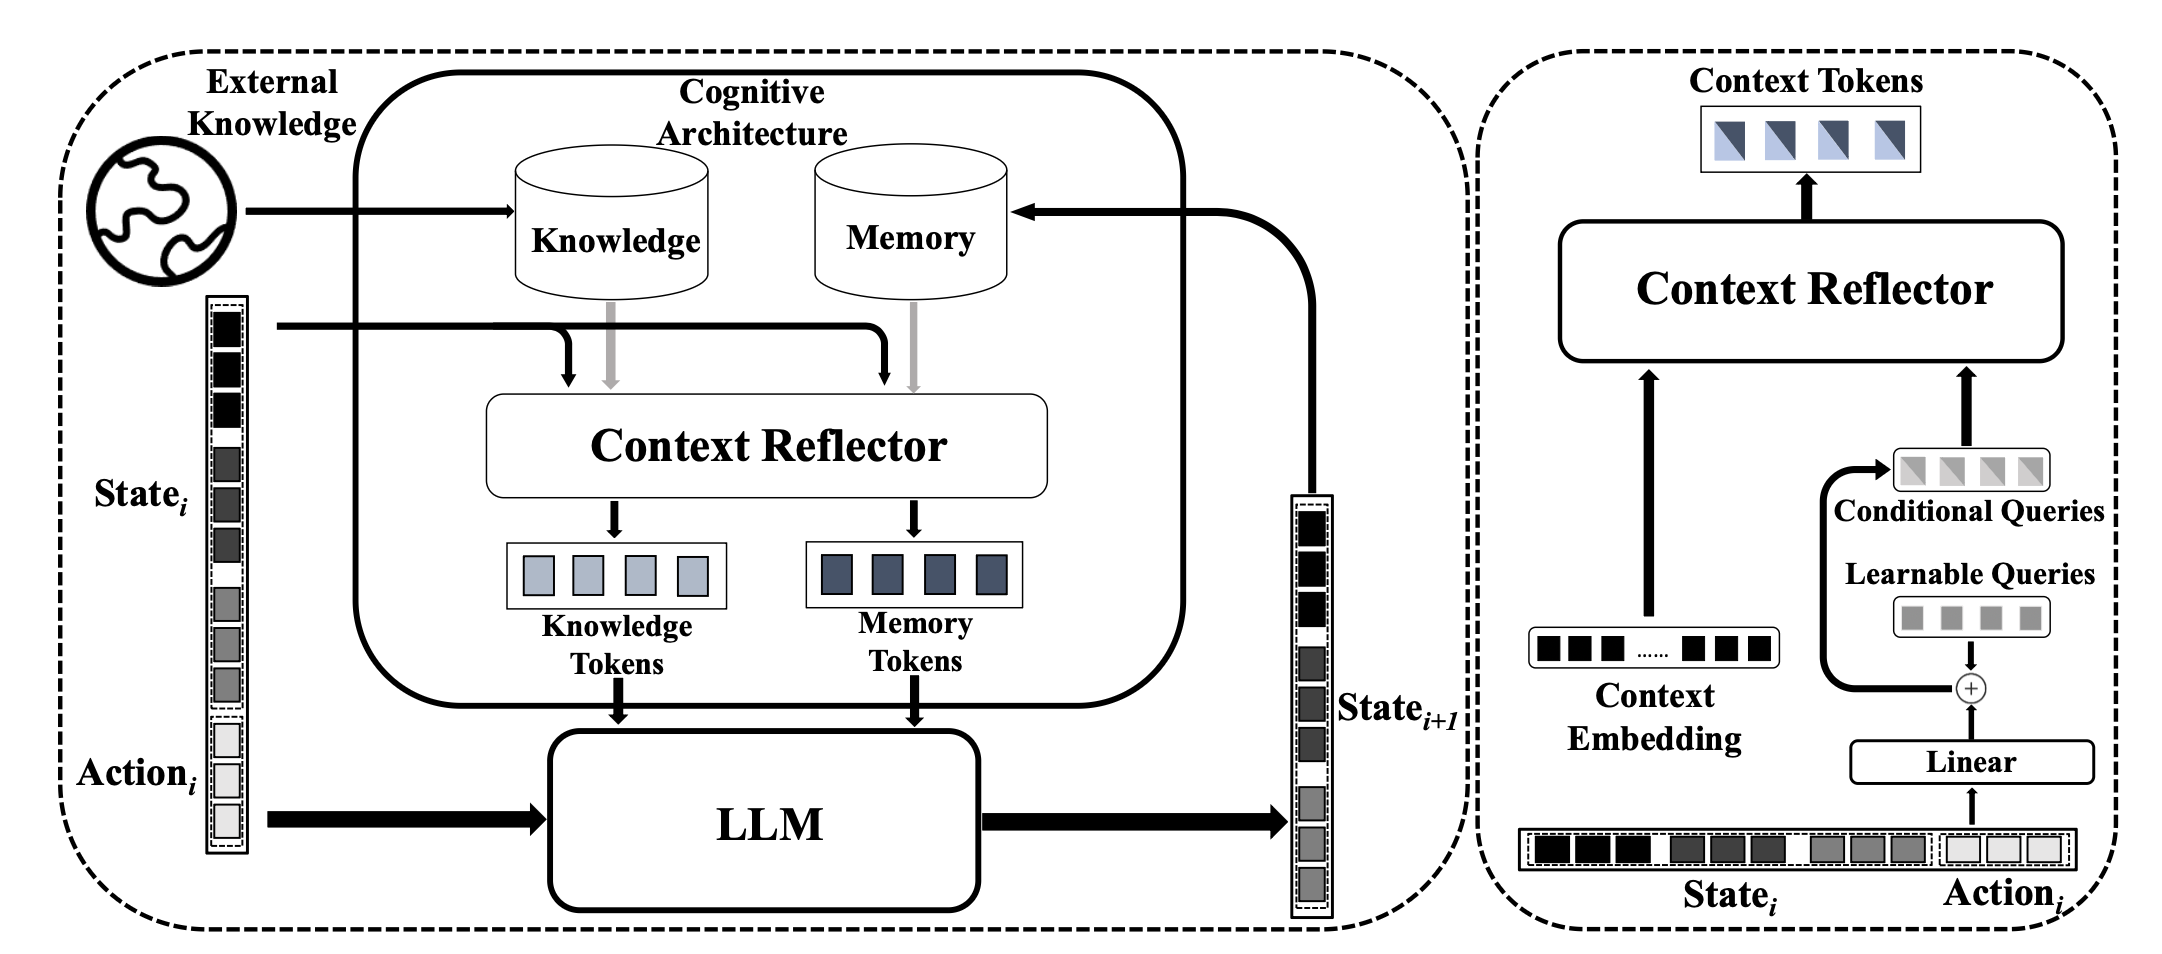
\includegraphics[width=0.95\linewidth]{figures/worldgpt}
    \caption{WorldGPT 的架构 \citep{ge2024worldgpt}}
    \label{fig:worldgpt}
\end{figure}


\paragraph{WorldGPT}
WorldGPT 基于标准 LLM Vicuna-7B-v0。\footnote{\url{https://huggingface.co/lmsys/vicuna-7b-v1.3}, \url{https://lmsys.org}} 它遵循基于模型的强化学习方法，在潜空间中推理。%WorldGPT follows the retrieval-augmented generation (RAG) approach  using external knowledge bases, and also using external (long term) memory, to augment LLM performance further, by addressing the state problem (Section~\ref{sec:state}). 
WorldGPT 的目标是成为世界真实动力学的模拟器——即强化学习中的转移函数与奖励函数。为此，该架构借助一种特殊架构来合成多模态指令实例。WorldGPT 的核心遵循常见的 VLM 架构：中央一个 LLM，外加一个多模态编码器与一个解码器。为帮助模型合成多模态指令，加入了一套认知架构来协助专门的或长期的任务。该架构增加了记忆、知识检索与上下文反思。上下文反思建立在 Q-former 之上 \citep{li2023blip}。架构图见图~\ref{fig:worldgpt}。

\paragraph{WebDreamer}
WebDreamer 面向 Web 交互。它把大模型 Qwen-70B \citep{bai2025qwen2} 蒸馏成一个小的 7B 模型。然后用小模型在"真实"Web 世界中行动之前，用世界模型模拟动作。它用模型预测控制（MPC）作为规划方法 \citep{garcia1989model,schwenzer2021review}，对网站动作做决策，并在每个交互步骤重新规划。WebDreamer 把 LLM 用作世界模型与价值函数。LLM 同时实现了
模拟函数（sim）与打分函数（score），见图~\ref{fig:webdreamer}。
此外，沿着 \citep{koh2024tree} 的思路，LLM 还被用于候选动作生成（除了 sim 与 score 之外）。作者
采用两阶段方法：先采样 top-$k$ 个动作，
然后用 LLM 自我精炼掉那些不必要模拟的动作。

\begin{figure}
    \centering
    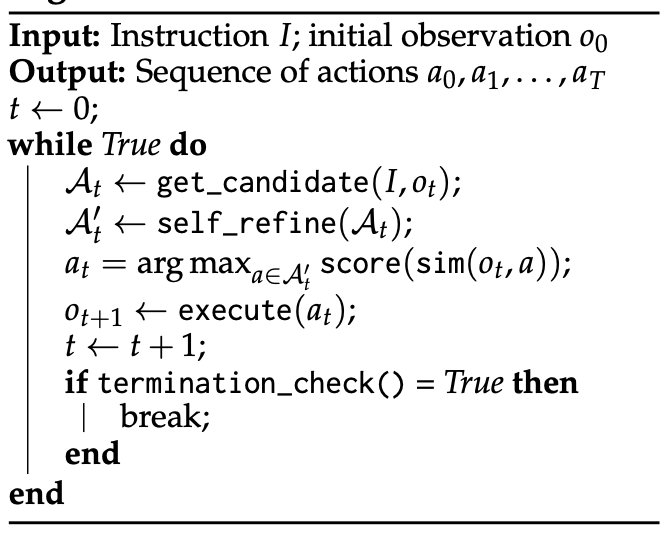
\includegraphics[width=0.5\linewidth]{figures/webdreamer}
    \caption{WebDreamer 伪代码：用 LLM 实现 score 与 sim 函数 \citep{gu2024your}}
    \label{fig:webdreamer}
\end{figure}

\paragraph{WorldCoder}
\begin{figure}
    \centering
    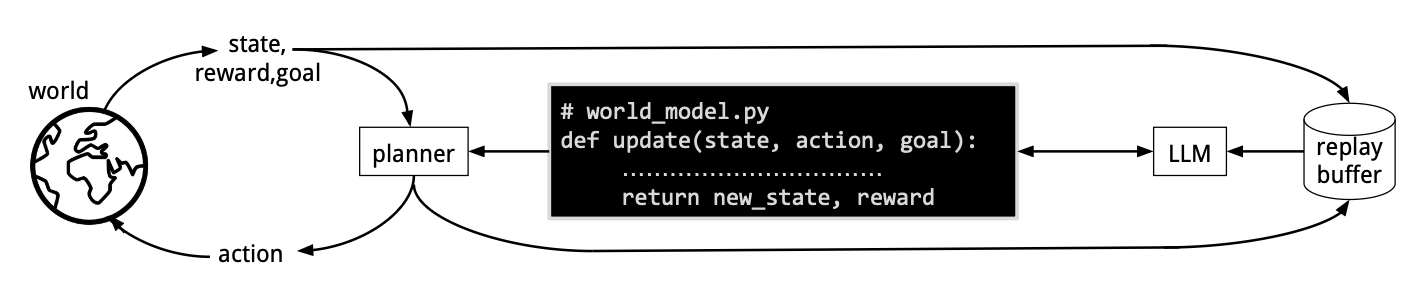
\includegraphics[width=0.95\linewidth]{figures/worldcoder}
    \caption{WorldCoder 架构 \citep{tang2024worldcoder}}
    \label{fig:worldcoder}
\end{figure}
WorldCoder 是一个基于模型的智能体，它构建一个 Python 程序来表示自己对世界的知识。WorldCoder 创建世界的转移函数，以可执行的 Python 代码呈现，见图~\ref{fig:worldcoder}。
WorldCoder 使用程序合成。% It is a model-based agent that builds Python functions to represent its world knowledge. 
在强化学习中，问题被形式化为 MDP，由状态表示 $S$、动作函数 $A$、转移函数 $T$ 与奖励函数 $R$ 构成（见第~\ref{sec:mbrl} 节）。WorldCoder 用 LLM 为一个任务生成动作、转移与奖励函数的 Python 代码，以及状态表示，然后把它用于基于模型的强化学习方法。这段代码会被检查和改进，经过迭代的自我调试精炼过程 \citep{chen2023teaching}，见第~\ref{sec:selfdebug} 节。
%The  world models are programs, so in each self-debug refinement iteration the LLM is prompted with the erroneous program it previously generated, together with state-action transitions
%that program cannot explain, and prompted to fix its code. 
这一过程反复进行，直到程序
产出正确输出。

请注意，在 WorldCoder 中学到的模型是符号化的（转移函数以计算机代码表示），而在常规深度强化学习中它是神经网络。在推理时，WorldCoder 是高效的，因为不需要调用 LLM 做大网络的前向传播，只需解释转移函数与奖励函数的 Python 代码。

在常规的基于模型的 LLM 方法中，LLM {\em 模拟}世界；而在 WorldCoder 中，LLM {\em 构建}一个世界的模拟，供后续执行。在推理时，由 Python 解释器执行转移函数；而在 ReAct 中，由 LLM 对世界状态做推理。对规划问题而言，符号化方法更合适，因为 LLM 在推理时做规划很吃力（见第~\ref{sec:knowing} 节）。

\subsection{学习算法}
下面我们讨论不同方法所用的预训练与微调算法。%Again, a reinforcement learning algorithm is used to learn from feedback.
%RAP  Uses MCTS for planning, with separate prompts for the LLM to use it for the MDP functions.

\paragraph{WorldGPT}
WorldGPT 通过在跨多个领域的数百万视频上预训练与微调，获得对世界
动力学的理解。以 Vicuna-7B-v0 作为基础 LLM。预训练随后使用以语言为中心的编码器，获得多模态状态的统一表示。对于多模态解码，会往 LLM 的词表中插入特殊词元。训练从单模态开始，逐步推进到跨模态。对于微调，使用一套特殊的认知强化架构，数据集带有来自超过 1000 万视频的细粒度顺序状态转移样本标注。如前所述，该认知架构由记忆、知识检索与上下文反思组成。通过微调，智能体通过在合成多模态指令数据上微调来获得专门知识。%\todo{wordt er RL gebruikt? PPO?}

\begin{comment}
!!!!!!!!!!!!!!!!!!!!!!!!!!!!!!!!!!!!!!!!!!!!
Ga de papers lezen en schrijf op hoe ze pretraining en finetuning doen.
En check ook architecture!!!!

WebDreamer Summary:
\begin{itemize}
    \item Goal: Be able to use LLM to simulate. Enable Model-based Planning for Web Agents before committing to real action. How can we build effective world models for the Internet? Unlike traditional
world models in RL focusing on improving data efficiency in the agent learning process,
LLM-based world models emphasize decision-making over simulation fidelity, leveraging
broad world knowledge for planning. 
    \item Data: finetune on 3.1 million interaction
instances. Data synthesis pipeline consists of (1) Web Random Walking,
where we autonomously interact with web pages through actions like typing for search
and clicking, and (2) Synthesis, where Qwen2-VL-72B (Wang et al., 2024) generates textual
descriptions of state changes based on visual snapshots before and after actions. 
    \item Arch: LLM as World Model and Value Function. To this end, we introduce WEBDREAMER, a model-based planning framework that uses LLMs to simulate and score possible future states before executing actions. WEBDREAMER leverages LLMs to implement
both the simulation function (sim) and the scoring function (score) (see Figure~\ref{figwebdreamer}).
    \item Learning: Train LLM with scalable data synthesis pipeline. Pretrained on web-scale data, finetune on 3.1 million interaction
instances. Uses MPC which simulates possible
future states for each action over a finite horizon. Implementation
of sim consists of two modules: one predicts
state changes after action execution, approxi-
mating the state transition function T, while the
other imagines a possible action based on the
predicted state to enable long-horizon planning.
Together, these two modules generate trajecto-
ries of length H. Next, use an LLM as a scoring function for each simulation. Furthermore, following \citep{koh2024tree}, LLM is used in addition to sim and score, for candidate action generation. They
employ a two-stage approach: first sampling top-k actions 
then using LLM to self-refine unnecessary actions for simulation.
    \item Results: substantial performance improvements over reactive baselines: 4-5 times more efficient than tree-search. Performance comparable to GPT-4o. competitive with the tree search method, while being 4–5
times more efficient on sandbox environment VisualWebArena, and performs effectively
on real-world websites (Online-Mind2Web and Mind2Web-Live), where tree search meth-
ods are difficult to implement and deploy. Moreover, Dreamer-7B achieves performance
comparable to GPT-4o on two online benchmarks. On Online-Mind2Web and Mind2Web-Live, WEBDREAMER
outperforms the reactive baseline by a relative gain of 42.3\% and 23.8\%, respectively. Another key advantage of model-based planning is its efficiency compared with
tree search using actual explorations. 
\end{itemize}
\end{comment}

\paragraph{WebDreamer} WebDreamer 方法的目标是学习适合基于模型的强化学习的动力学。首先用预训练的 Qwen-2-VL 视觉语言模型 \citep{wang2024qwen2} 初始化 Dreamer-7B 模型，然后在 310 万个交互样本上进一步微调。
数据合成流水线由两部分组成：（1）在 Web 上随机漫游，
即模型通过诸如输入搜索词、
点击之类的动作自主地与网页交互；（2）合成，即由 Qwen2-VL-72B 根据动作前后的视觉快照生成状态变化的文字
描述。WebDreamer 在有限的时间跨度上模拟每个动作可能的
未来状态（按照模型预测控制（MPC）方法重新规划与重新训练，MPC 是一种用于自适应重训练的强化学习方法，常用于工程与控制问题）。


\paragraph{WorldCoder}
WorldCoder 使用程序合成来学习构建转移函数——那个计算世界下一状态的函数。WorldCoder 随后用这个编码后的世界模型执行规划动作。它最初
执行随机探索来初始化一个环境交互数据集；它用一个程序合成算法更新自己的世界
模型、生成代码，然后
执行规划。可以使用不同的规划器，从深度受限的值迭代（在
简单域中）到 MCTS（在更复杂的域中）\citep{browne2012survey}。
%combinatorial program synthesis. Explore the space of possible programs.


\begin{comment}
WorldCoder Summary:
\begin{itemize}
    \item Goal: World-coder is a model-based agent that builds a Python program to represent its knowledge of the world, a transition function of the world in executable Python code, see Figure~\ref{fig:worldcoder}. In principle the same knowledge as a regular (non-executable) model, although the WorldCoder model can be run standalone outside a supporting system, and adds options in use and transfer of knowledge. Since WorldCoder can edit its own code, similar to self-reflection in regular (non-executable) models, and it can use this capability to transfer knowledge across environments (generalization). In addition, WorldCoder tries to explain its interactions.

    An important difference between WorldCoder is that the learned model is symbolic (computer code), where in regular deep learning models the model is a neural network. At inference time, WorldCoder is efficient, since no LLM calls occur, just interpretation of the trainsition and reward function code.

    In regular model-based LLM approaches, the LLM simulates the world, in WorldCoder the LLM {\em builds} a simulation of the world, for later execution. At inference time, the Python interpreter executes the transition function, where in ReAct, an LLM reasons about the world state. LLMs struggle with planning during inference, WorldCoder plans easily.
    \item Data:
    \item Arch: an architecture that
synthesizes a Python program to model its past experiences with the world, effectively learning the
transition function
    \item Learning: Learn to make a transition function, the function that predicts the next state of the world. takes actions by planning using that world model. combinatorial program synthesis. Explore the space of possible programs.
    \item Results: world models have many advantages: they allow reasoning in radically new situations
by spending more time planning different actions, and accomplishing novel goals by just changing
the reward function. WorldCoder is tried on gridworlds, and on task planning, finding the approach is more sample-efficient compared to model-free deep reinforcement learning, and more compute-efficient compared to fully-prompt-based ReAct-style agents, and that it can transfer its knowledge across environments by editing its code. 

Sokoban, Minigid, and AlfWorld



Representing world knowledge as code, and generating it from LLMs, brings
other advantages. It allows prior world knowledge embedded in the LLM to inform code generation,
allows sample-efficient transfer across tasks by reusing pieces of old programs, and allows auditing
the system's knowledge, because programming languages are designed to be human-interpretable.

Though promising, a limitation of the WorldCoder approach is inherent to the computational difficulty of many of the planning problems that it is applied to. Problem instances of combinatorial puzzles such as Sokoban that are difficult to solve with dedicated solvers, will also be difficult to solve for WorldCoder. The transition function that is generated by the LLM is unlikely to be better than those designed by expert human researchers. On the other hand, the LLM may well have seen such codes during pretraining, and the generated transition function may come close, for such problems.

So far, the synthesized  code aims to reproduce the transition and reward functions. Self reflection and metalearning approaches may be able to improve performance further.
\end{itemize}
\end{comment}

%Different planners are suggested for WorldCoder, such as depth-limited value iteration (in simple domains) and MCTS (for more complex domains).



\subsection{结果}
下面我们看这三种方法的结果。
%RAP works on planning blocksworld, math question answering.

\paragraph{WorldGPT} WorldGPT 模型用一个多模态状态转移预测基准来评估。WorldGPT 是有效的，它能准确理解并预测复杂现实厨房与烹饪场景的动态。
%of  real-life scenarios. Evaluations
%on WorldNet directly demonstrates WorldGPT's capability to accurately model state transition patterns, 
%affirm its effectiveness in understanding and predicting the dynamics of complex scenarios. 

该系统还作为世界模拟器做过评估，结果表明%the synthesis of multimodal instructions allows 
它能泛化到不熟悉的领域。
在一项实验中，WorldGPT 在音视频问答
任务上比传统基于扩散的方法快 30 倍
\citep{ge2024worldgpt}。

\paragraph{WebDreamer} WebDreamer 表现也不错。据报道，它在 Web 交互任务上超越了 GPT-4o 的表现。
相比反应式基线，报告了显著的性能提升，在树搜索上效率高 4–5 倍。WebDreamer 在沙盒环境 VisualWebArena 上表现良好，在真实网站（Online-Mind2Web 与 Mind2Web-Live）上也表现不错，而这些地方树搜索方法难以实现与部署。此外，在在线基准上，使用 Dreamer-7B，该方法取得了
与 GPT-4o 相当的表现。在真实网站上，WebDreamer
分别以 42\% 和 24\% 的相对增益超越反应式基线。%Another key advantage of model-based planning is its efficiency compared with tree search using actual explorations. 

\paragraph{WorldCoder} 
WorldCoder 的结果在网格世界与任务规划（AlfWorld）上有报告。WorldCoder 比无模型强化学习样本效率更高，与试图由 LLM 做上下文规划的 ReAct 式智能体相比算力效率更高。%, and that it can transfer its knowledge across environments by editing its code.

% The WorldCoder system assumes deterministic dynamics and requires symbolic state representations. WorldCoder is tried on gridworlds, and on task planning, finding the approach is more sample-efficient compared to model-free deep reinforcement learning, and more compute-efficient compared to fully-prompt-based ReAct-style agents, and that it can transfer its knowledge across environments by editing its code. 
% Sokoban, Minigid, and AlfWorld

用 LLM 把世界知识生成为计算机代码会带来
好处。它使 LLM 中嵌入的先验世界知识能改善代码生成，因为已发表问题的现成解法很可能在预训练中见过。这些代码还可以通过复用旧程序的片段跨任务迁移。此外，结果是人类可读的，使人能通过阅读生成的代码来检查世界知识。
%auditing the system's knowledge, because programming languages are designed to be human-interpretable.

尽管对规划问题而言很有前景，WorldCoder 方法的一个局限源自规划问题固有的计算难度。用专用求解器都难以求解的问题实例，对 WorldCoder 求解器同样困难。LLM 生成的转移函数不太可能优于专业人类研究者设计的那些。%On the other hand, the LLM may well have seen such codes during pretraining, and the generated transition function may come close, for such problems.

迄今为止，合成的代码旨在复现转移函数与奖励函数。未来工作中，自我反思与元学习方法或许能进一步提升性能。



\subsection{*基于模型的强化学习}\label{sec:mbrl}





\begin{comment}
    
World models are being used successfully in agentic LLM. An extensive literature exists on world models in model-based reinforcement learning. At the end of this chapter, we will now provide a brief overview of world models in model-based reinforcement learning, in order to provide more context for the use of world models  in LLM. 
\end{comment}

世界模型正被成功地用于智能体大语言模型。关于基于模型的强化学习中的世界模型，已有大量文献。在本章末尾，我们现在简要综述基于模型的强化学习中的世界模型，以便为世界模型在 LLM 中的使用提供更多背景。

一个有影响力的早期基于模型的方法是 Dyna \citep{sutton1991dyna}。有影响力的近期工作有 \citep{ha2018world,hafner2020mastering}。两篇现代综述是 \citet{moerland2023model,plaat2023high}。

在强化学习中，智能体通过采样环境中执行动作所得的奖励，来学习如何在
环境中行动。% (see Figure~\ref{fig:rl7}). 
%
%
% \begin{figure}
%   \begin{center}
%     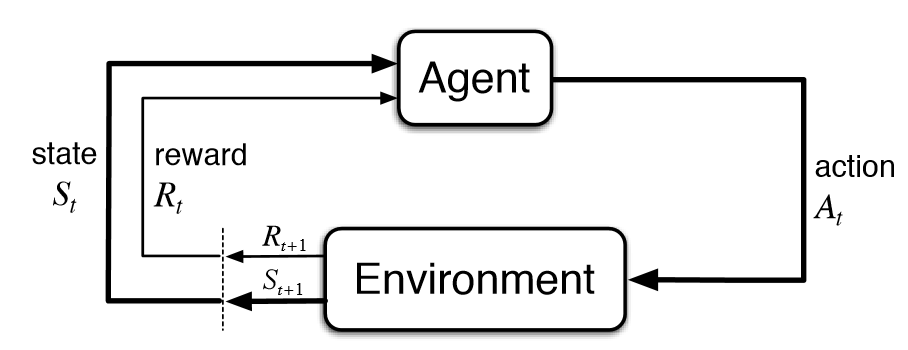
\includegraphics[width=9cm]{figures/rl}
%     \caption{Reinforcement Learning: Agent acting in Environment \citep{sutton2018reinforcement}}\label{fig:rl7}
%   \end{center}
% \end{figure}
%


%World models have been successful in learning robotic movement in complex environments, to play Atari video games, and to act in open world games such as MineCraft \citep{hafner2020mastering,hafner2023mastering}.
%World models can also be
%trained effectively with LLMs \citep{ge2024worldgpt}. 
%For example, WorldCoder builds a world model as a Python program from
%interactions with the environment \citep{tang2024worldcoder}. The world model explains its
%interactions with a language model.

%Make a new model, to use as input, new training data.

%While world models are mostly associated with reinforcement learning,
%they are also used to generate a model in planning domains (blocks-world) in PDDL, to aid task-planning \citep{guan2023leveraging},
%achieving success in ALFWorld \citep{shridhar2020alfworld}.


% Can VLAs help take actions?
%Agents can learn a policy to act with reinforcement learning from surrogate world models. However, agents can also learn action models directly. 
%
%New models to train on.
%Three examples are
%\citet{ahn2022can,radford2021learning,suglia2021embodied}, who ground
%language models in world models of robotic actions. 
%\citet{xiang2024language} use world models to finetune language models
%to gain diverse
%embodied knowledge while retaining their general language capabilities.

\begin{figure}
  \begin{center}
    \input figures/rl
    \caption{标准强化学习循环。智能体从环境给出的反馈奖励 $r$ 中学习一个 $\theta$ 参数化的策略 $\pi_\theta$。\citep{sutton2018reinforcement}}\label{fig:rl7b}
  \end{center}
\end{figure}

\subsubsection{无模型强化学习}
在常规强化学习中，最优智能体策略是以无模型方式学到的：所有状态下的最佳动作直接从与环境的交互中学到（见图~\ref{fig:rl7b}），不借助任何额外的环境模型。常规强化学习被形式化为马尔可夫决策过程，包含四个函数 $\{S, T, A, R\}$：函数 $S(o)\rightarrow s$ 为观测 $o$ 表示系统状态，函数 $T(s,a)\rightarrow s'$ 用动作从一个状态转移到下一个状态，函数 $A(s)\rightarrow a$ 为某个状态返回一个动作，函数 $R(s)\rightarrow r$ 为状态赋予一个奖励值（正或负）。强化学习的目标是用 MDP 学出最优策略 $\pi^*(s)\rightarrow a^*$，即为 MDP 可能处于的每个状态返回最佳动作的函数。因此，一个强化学习问题由四个函数 $S$、$T$、$A$、$R$ 构成，智能体的目标是找到期望累积奖励最高的最优策略 $\pi^*(s)$。智能体无法访问 $T$ 与 $R$——这两个函数驻留在环境中。%If the agent wants to know if action $a$ is a good action, the so-called {\em policy evaluation} problem, then it has to perform action $a$ in the environments, which uses $T$ to transition to new state $s'$ and $R$ to compute the reward value $r$ of that new state, and return $(s', r)$ to the agent. The agent then uses $r$ to update the value for the action in the policy, the so-called {\em policy improvement} step.
常规的、无模型的强化学习也称为{\em 直接}强化学习。%The agent samples that environment, and improves the policy with feedback on each action. 
直接方法天然具有很高的样本复杂度：策略改进需要采样，而大型 MDP 需要大量样本才能使策略改进过程收敛（图~\ref{fig:rl7b}）。

%Now, when the real environment is too complex, executing those actions in the real environment may be too expensive, and learning the policy takes too long. In that case, agents may learn an extra, smaller, world model as a surrogate, locally. Accessing this local surrogate model is assumed to be cheap. They can then use this local model of the dynamics of the world to allow sample efficient training of the policy.  Such local world models are learned on the fly by model-based reinforcement learning from the environment interaction, concurrent to policy learning. Thus, each environment sample updates both the policy $\pi$ and the local model $M=(T', R')$.

\begin{figure}[ht]
  \begin{center}
    \input figures/mbrl
    \caption{基于模型的强化学习：环境反馈被用于同时改进策略 $\pi$ 与局部动力学模型 $\hat{M}=(\hat{T},\hat{R})$，而策略 $\pi$ 也从该模型采样（{\em 规划}）}\label{fig:mbrl}
  \end{center}
\end{figure}

\subsubsection{基于模型的强化学习}
在直接强化学习中，采样到的信息不被智能体保留，而是被遗忘，每次策略改进都需要新的样本。智能体与外部环境的交互往往代价高昂，例如在现实世界中行动的机器人，其关节会磨损。在这种情况下，想办法降低样本复杂度是有益的。我们应当设法不必向环境采样那么多也能改进策略。

一个直接的想法是不把样本扔掉，而是存进一个缓冲区，从这份旧交互结果缓冲区中采样；或者稍进一步，训练一个环境动力学的{\em 局部代理模型} $M=(\hat{T}, \hat{R})$。当我们训练好这个局部动力学模型后，除了向环境（昂贵地）采样，也可以（廉价地）从模型采样（见图~\ref{fig:mbrl}）。

这些方法是间接方法，因为在最后这类方法中，局部动力学模型由智能体自己构建，策略是从环境中间接（经由局部模型）学到的。

使用局部动力学模型称为基于模型的强化学习。动力学模型由智能体对真实 $T$ 与 $R$ 的局部估计 $\hat{T}$ 与 $\hat{R}$ 构成，而真实的 $T$ 与 $R$ 只有环境知道。
基于模型的强化学习已在一些应用中取得成功，例如围棋 \citep{silver2016mastering}、 Diplomacy \citep{meta2022human}、星际争霸 \citep{vinyals2019grandmaster}，以及跨领域学习 \citep{hafner2020mastering}。


基于模型的强化学习还与{\em 规划}相关——规划是符号人工智能中的一个经典领域，它通过高效的潜表示模拟不同的可能世界来展望未来，而不必在真实世界中行动。

\subsubsection{降维}
在深度基于模型的强化学习中，局部动力学模型也称为世界模型 \citep{ha2018world}。
在这一语境下，世界模型把高维观测空间降为低维状态空间与奖励空间，然后可用于基于模型的强化学习方法，以高效改进策略函数。
%, that sample from the low-dimensional dynamics model.
其背后的想法是：在大多数高维环境中，
存在一些不那么重要的元素，例如电子游戏中背景里
从不移动的树，它们与动作价值
几乎没有关系。目标是
把输入空间中这些
不重要的元素抽象掉，
降低状态空间的有效维度。

\subsubsection{联合嵌入预测架构}
联合嵌入预测架构（JEPA）由 \citet{lecun2022path} 提出，并在 \citet{assran2023self} 中进一步完善。JEPA 的目标是在抽象的、压缩的表示（潜空间）中预测未来状态，而不是试图重建原始的感官细节或像素。这一目标与基于模型的强化学习中世界模型的降维目标相似。基于模型的强化学习学习一个由奖励监督的局部转移模型，而 JEPA 是一个自监督的表示学习框架。
JEPA 通过自监督观测（看视频或图像）来训练，把上下文嵌入映射到目标嵌入，不使用奖励或显式动作。基于模型的强化学习则明确纳入动作、奖励与控制优化，以最大化回报 \citep{lim2026jedi}。JEPA 与强化学习很接近，JEPA 可以作为强化学习或规划算法的感知引擎（世界模型），例如用于引导机器人控制 \citep{destrade2025value}。


\begin{comment}
!!!!!!!!!!!!!!!!!!!!!!!!!!!!!
En nu world model gaan noemen. En dat een LLM een world model is, en met fine tuning online verbeterd wordt door interactie. ICRL kan dan samplen van het world model (het LLM) om de optimale policy te bepalen. acties.

\todo{Sectie herschrijven. Er is nog geen lijn. Eerst logische lijn maken} The agent improves its policy of best actions for each state from the reward that an outside environment provides, see Figure~\ref{fig:rl7}. After using the reward for updating the policy, it is thrown away, and new rewards are sampled from the environment. This model works when environment interaction is cheap, but when it is expensive, then it might be more advantageous to remember the rewards, and have the agent build its own model of the environment, from which the agent can then also take (cheap) samples to as it is improving its policy function. This approach is called model-based reinforcement learning \citep{moerland2023model,plaat2023high}, and it has been successful in some applications, such as Go \citep{silver2016mastering}, Diplomacy \citep{meta2022human}, StarCraft \citep{vinyals2019grandmaster}, and showing learning accross domains \citep{hafner2020mastering}. The locally learned models learn the transition function and the reward function. Together, they are  called the dynamics model, since it models the dynamics of the environment. The models are also called world models. World models are an important factor in the success of agents. 


 Recall that the environment
samples return $(s',r')$ pairs when the agent selects action $a$ in
state $s$. This means that  we can learn the
transition model $T_a(s,s')$ and the reward model $R_a(s,s')$, for
example by supervised learning, since
all necessary information is present. When the transition and reward model are
present in the agent, they can then be  used with planning to update
the policy and value functions as often as we like \emph{without any
  further sampling of the environment} 
(although we might want to continue sampling to further improve our
models). This
alternative approach  
of finding the policy and the value is called model-based learning,
see Algorithm~\ref{lst:back} and Figure~\ref{fig:learn}. 



\begin{figure}[t]
  \centering
    \input figures/learn
    \caption{Model-Based Reinforcement Learning}\label{fig:learn}
  
\end{figure}




\begin{figure}[t]
  \begin{center}
    \input figures/imagination
    \caption{Dyna's Model-Based Imagination}\label{fig:imagination}
  \end{center}
\end{figure}



%
%
\begin{algorithm}[t]
  \begin{algorithmic}
    \Repeat
    \State Sample env $E$ to generate data $D=(s, a, r', s')$ 
    \State Use $D$ to learn $T_a(s,s')$ and  $R_a(s,s')$ 
    \State Use $T, R$ to update policy $\pi(s, a)$ by planning 
    \Until $\pi$ converges
  \end{algorithmic}
  \caption{Model-Based Reinforcement Learning}\label{lst:back}
\end{algorithm}

% If the model is given, then no environment samples are needed and 
% model-based methods are  more sample efficient. But if the
% model is not given,
Why would we want to go this convoluted learning-and-planning route,
%which may even introduce model-bias,
if
the environment samples can teach us the optimal policy and value directly? The
reason is that the convoluted route may be more sample efficient.

In model-free learning
a sample is used once to optimize the policy, and then thrown away,
while in
model-based learning 
the sample is used to learn a transition model, which can then be used many
times in planning to optimize the policy. The sample is
used more efficiently by the agent.
 
A well-known classic model-based approach is \emph{imagination}, which was
introduced by~\citet{sutton1990integrated,sutton1991dyna} 
in the Dyna system, long before deep learning was used widely. 
%Dyna uses the environment samples to update the policy  function directly (model-free learning) and also uses the samples to learn a transition model,  to augment the model-free environment-samples with the model-based imagined ``samples.'' % In this way the sample-efficiency of model-free
% learning is improved quite directly.
%Imagination is a hybrid algorithm that uses both model-based planning and model-free learning to improve the behavior policy.
% , with the creation of these imagined planning updates.
%Figure~\ref{fig:imagination} illustrates
%the working of the Dyna approach.
%Algorithm~\ref{lst:dyna} shows the
%steps of the algorithm (compared to  Algorithm~\ref{lst:back}, the
%line in italics is new, from Algorithm~\ref{lst:free}). Note how the
%policy is updated twice in each iteration, by environment sampling, and by
%transition planning. More details are shown in Algorithm~\ref{alg:dyna-q}~\citep{sutton1990integrated}.


\begin{algorithm}[t]
  \begin{algorithmic}
    \Repeat
    \State Sample env $E$ to generate data $D=(s, a, r', s')$ 
    \State {\em Use $D$ to update policy $\pi(s, a)$}
    \State Use $D$ to learn $T_a(s,s')$ and  $R_a(s,s')$ 
    \State Use $T, R$ to update policy $\pi(s, a)$ by planning 
    \Until $\pi$ converges
    \end{algorithmic}
    \caption{Dyna's Model-Based Imagination}\label{lst:dyna}
\end{algorithm}

% Dyna was introduced for a tabular approach before deep learning
% became popular. In Dyna,  the transition model is updated directly
% with samples.
%Note that the policy network is now updated twice in each iteration,
%once with 
%environment samples, and once with the  planning data.
%
% learn the policy without direct environment
% samples for the policy. In Dyna  the model-free lookahead planning is
% called ``imagination.'' In contrast to the previous section, in Dyna
% the same method is used for optimizing the policy
% from real experience as from imagined experience, generated by planning.






\begin{algorithm}[t]
  \input figures/dynaq
  \caption{Dyna-Q: Classic learning and planning with a Q-function-based dynamics model~\citep{sutton1990integrated}} 
  \label{alg:dyna-q}
\end{algorithm}

The principles of Dyna have been developed further in various directions, which we will now discuss.



The principles of Dyna have been developed further in various directions, which we will now discuss.


%\subsection{World Models !!TOTAL REWRITE!!}
\todo{No, essence of world models is not high dimensionality, essence is a local copy of the environment to learn more efficiently from. Talk about planning (Dyna) and then Dreamer}
A major challenge in machine learning that has been addressed by deep learning is to model high dimensional problems. In reinforcement learning, World models do so in model-based reinforcement learning. 
%\todo{Yes, but in model free also deeo learniing} 
World models reduce high dimensional observation spaces to lower dimensional state and reward spaces, that can then be used in model-based reinforcement learning methods to efficiently improve policy functions, that sample from the low-dimensional dynamics model.
The idea
behind world models is that in most high-dimensional environments
there are elements that are less important, such as background trees
that never move,  that have little or no relation with the reward
of the agent's actions. The goal  is to
abstract away these  unimportant elements of the input space, 
reducing the effective dimensionality of the space. 
%!!!!!!!!!!!!!!!!!!!!!!
World models do so by
learning the relation between the elements of the input and the
reward  either by auto encoding or with supervised learning
conditioned on value.  %When we focus our learning mechanism  on the changes in observations that are correlated with changes in these values, then we can improve the efficiency of  learning high-dimensional problems greatly.
%Unimportant elements (such as background trees that never move) have
%a weak relation with the reward, and they are abstracted away.
World models thus learn a smaller representation, smaller than the
observation space.
Planning  takes place in this smaller representation space.



% It turns out that in high-dimensional input scenes
% typically only a few objects influence the reward, and many elements
% are irrelevant. 
% Think of images of landscapes in which a character
%moves, where trees in the background do not influence the score, or
%images of a robot-arm, where a desk  in the background never
%moves, and similarly does not influence the reward of the action to
%be learned.


%In an early example of world models, the  value prediction network (VPN), introduced by ~\citet{oh2015action,oh2017value}, 
%to achieve this goal. They 
%ask the question in their paper: ``What if
%we could predict future rewards and values directly without predicting
%future observations?'' and 
%describe a network architecture and learning
%method for models focused on value prediction. The core idea is not to
%learn directly in actual observation space, but 
%first to
%transform the actual state representation to a smaller latent representation
%model, also known as abstract model. 
%The other functions, such as
%value, reward, and next-state, then work with the smaller latent representations,
%instead of the actual high-dimensional states. By training all functions based on the
%values, planning and learning occur in a space
%where states are encouraged only to contain the elements that influence
%value changes. % Non-essential elements, such as trees, houses, or other
% unchanging background, are not part of the latent states.
%We will now explain the latent-model approach using VPN.\footnote{See
%  \url{https://github.com/junhyukoh/value-prediction-network} for the code.}
%In VPN the world model consists of four networks: an (LSTM) encoding
%function, a reward function, a value function, and a transition
%function. All functions are parameterized with their own set of
%parameters (Figure~\ref{fig:oh}).
%
%Latent space is lower-dimensional, and training and planning become more efficient.
%The figure shows a single step rollout, planning one step ahead, 
%as in Dyna-Q (Algorithm~\ref{lst:dyna}).

% To distinghuish these latent-based functions from the
% conventional observation-based functions $R, V, T$ we denote them
% differently as $f^{enc}_{\theta_e}, f^{reward}_{\theta_r},
% f^{value}_{\theta_v}, f^{trans}_{\theta_t}$.

% \begin{itemize}
% \item The encoding function $f^{enc}_{\theta_e}:s_{actual}\rightarrow
% s_{latent}$ maps the observation $s_{actual}$ to the abstract state
% using a neural network $\theta_e$, such as a CNN for visual observations.
% \item The latent-value function
%   $f^{value}_{\theta_v}:s_{latent}\rightarrow
%   V_{\theta_v}(s_{latent})$ maps the abstract state to its value using
%   a separate neural network $\theta_v$. This value is the value of the
%   latent state, not of the actual observation state $V(s_{actual})$.
% \item The latent-reward function $f^{reward}_{\theta_r}:(s_{latent},o)\rightarrow r,
% \gamma$ maps the latent state and option (a kind of action) to the
% reward and discount factor. If the option takes $k$ primitive actions,
% the network should predict the discounted sum of the $k$ immediate
% rewards as a scalar. (The role of options is more fully explained in the paper.) The network also predicts option-discount factor
% $\gamma$ for the number of steps taken by the option.
% \item The latent-transition function $f^{trans}_{\theta_t}:(s_{latent},o)\rightarrow
%   s'_{latent}$ maps the latent state  to the next latent state,
%   depending also on the option.
% \end{itemize}
% Figure~\ref{fig:oh} shows how the function work together, with $x$ the
% observed actual state, and $s$ the encoded latent
% state~\citep{oh2017value}. 



 %\begin{figure}[t]
 %\begin{center}
 %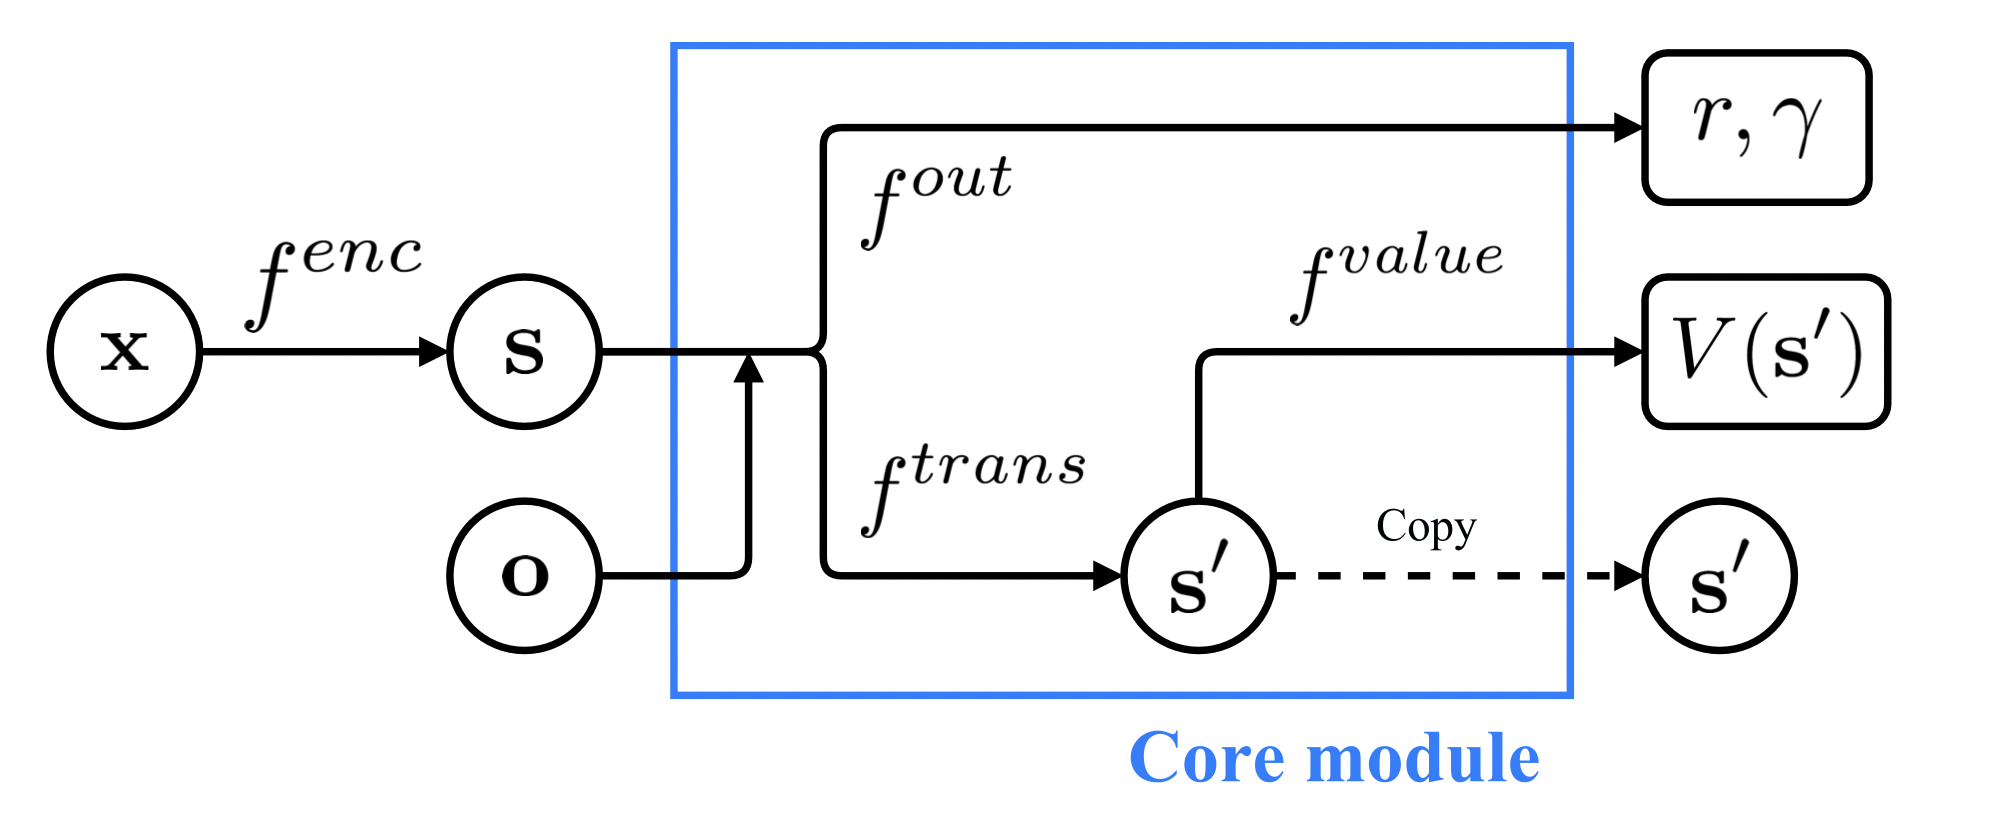
\includegraphics[width=7cm]{figures/oh2017core}
 %\caption{Architecture of world model VPN~\citep{oh2017value}}\label{fig:oh}
 %\end{center}
 %\end{figure}


% , where the model was used for
% single step sampling, just as the environment. Howerver, in contrast to an
% environment, a model also allows looking further into the future, by
% performing multi-step rollouts. Of course, this requires a highly
% accurate model, otherwise the accumulated inaccuracies diminish the
% value of the far-into-the-future lookahead. Algorithm~\ref{alg:dplan}
% shows the pseudocode for a $d$-step planner for the value prediction
% network.
% % \footnote{
% %The Q-value in the pseudocode is calculated as
% %$Q_\theta^d(s,o)=r+\gamma V^d_{\theta}(s')$ where
% %$V^d_\theta(s)=\frac{1}{d}V_\theta(s)+\frac{d-1}{d}\max_o
% %Q_\theta^{d-1}(s,o)$  and if $d=1$ then $V_\theta^d(s)=V_\theta(s)$.}


% \begin{algorithm}

%   \begin{algorithmic}
%             \Function{Q-Plan}{s, o, $d$}
%             \State  $r, \gamma, V(s'), s' \rightarrow
%             f^{core}_\theta(s, o)$ \Comment{Perform the four latent functions}
%             \If{$d=1$}
%             \State \Return{$r+\gamma V(s')$}
%             \EndIf
%             \State $A\leftarrow b$-best options based on $r+\gamma
%             V_\theta(s')$ \Comment{See paper for other expansion strategies}
%             \For{$o'\in A$}
%             \State $q_{o'} \leftarrow $ Q-Plan$(s',o',d-1)$
%             \EndFor
%             \State \Return{$r+\gamma[\frac{1}{d}V(s')+\frac{d-1}{d}\max_{o'\in
%                 A} q_{o'}]$}
%         \EndFunction
%   \end{algorithmic}
%   \caption{Multi-step planning~\citep{oh2017value}}\label{alg:dplan}

% \end{algorithm}

%The training of the networks can in principle be performed with any
%value-based reinforcement learning algorithm. \citet{oh2017value} report results
%with $n$-step Q-learning and temporal difference search~\citep{silver2012temporal}.
%In
%general, trajectories are generated with an $\epsilon$-greedy policy
%using the planning algorithm from Algorithm~\ref{alg:dplan}.
%VPN~\citep{oh2017value} showed impressive results on Atari games such as Pacman
%and Seaquest, outperforming model-free DQN~\citep{mnih2015human}, and outperforming
%observation-based planning in stochastic domains.
%Subsequently, many other works have been published that further
%improved
%results~\citep{kaiser2019model,hafner2018learning,hafner2019dream,hafner2020mastering,sekar2020planning,silver2017predictron,ha2018world}.
%Many of these world-model approaches are complicated designs, with
%multiple neural networks, and different learning and planning algorithms.


% {\bf 
% Dit moet beter, dit is niet te volgen en vaag. Het gaat er om om
% algemene principes uit te leggen.
% } 

%In the next section we will discuss the performance of latent models.
In an influential early work, ~\citet{ha2018world} describe how world models are inspired
by the manner in which humans are thought to construct a mental model of
the world in which we live. Originally, world models were often
represented as recurrent neural networks that were trained using a variational
autoencoder~\citep{kingma2013auto,kingma2019introduction,goodfellow2014generative}. Later, transformer architectures were used, that were trained self-supervised. 
%They  learn a compressed spatial and temporal
%representation of the environment. In world models  multiple neural
%networks are used, for  a vision model, a
%memory model, and a controller~\citep{ha2018world}. By using features extracted from
%the world model as inputs to 
%the agent, a compact and simple policy can be trained to solve a
%task, and planning occurs in the compressed or simplified world. World
%models have been applied by~\citet{ha2018recurrent,ha2018world} on a
%car racing game~\citep{kempka2016vizdoom}.
The term
\emph{world model} %actually 
goes back to 1990~\citep{schmidhuber1990making}. 
%Latent models are  related to dimensionality
%reduction~\citep{van2009dimensionality}.
%Some ideas have to wait a
%long time before their time has come.

%{\bf is there a large sample complexity reduction?}



% The role of latent models in image-based reinforcement learning can be
% compared with the attention mechanism in natural language processing.
% In natural language processing the concept of attention has been quite
% important. Attention~\citep{sutskever2014sequence,cho2014learning} uses
% an encoder-decoder RNN mechanism  to improve the performance  machine
% translation.   Together with the
% subsequent development of transformer models, attention has caused breakthrough
% results such as the large language models GPT-2 and
% 3~\citep{devlin2018bert,radford2018improving,radford2019language,brown2020language}. 



% {\bf dit verhaaltje hieronder is fout, de crux is niet dat het meerdere functies zijn, maar dat het een compactere representatie van de observaties is}

% Latent models are born out of this need for
% more accurate predictive deep models. Latent models replace the
% single transition model with separate, smaller, specialized, representation models,
% for the different functions in a reinforcement learning algorithm. All
% of the elements of the MDP-tuple  may now get their own
% model. Planning occurs in latent space.


% Traditional deep learning  models represent
% input states directly in a single model: the layers of neurons and filters are all
% related in some way to the input and output of the domain, be it
% an image, a sound, a text or a joystick action or arm movement. All of
% the MDP functions, state, value, action, reward, policy, and discount, act on
% this single model. Latent models, on the other hand, are not connected
% directly to the input and output, but are connected to other
% models and signals. They do not work on direct representations, but on
% latent, more compact, representations. The interactions are captured in three to four
% different models, such as observation, representation, transition, and
% reward models. These may be smaller, lower capacity, models. They may be trained with
% unsupervised or self-supervised deep learning such as variational autoencoders~\citep{kingma2013auto,kingma2019introduction} or
% generative adversarial networks~\citep{goodfellow2014generative}, or recurrent networks.
% Latent models use multiple
% specialized  networks, one for each function to be
% approximated.



% Figure~\ref{fig:abstract} illustrates the abstract (latent) learning
% process (using the modules of 
% Dreamer~\citep{hafner2019dream}  as an example).
% %
% \begin{figure}[t]
%   \begin{center}
%     \input abstract
%     \caption{Latent Models}\label{fig:abstract}
%   \end{center}
% \end{figure}

% \subsubsection{CNN}
% Only in the context of e2e, of a network to learn the transition
% function, and at the same time the planning function

% {\bf En wat moet ik hier dan vertellen???}
The architecture of world models is elaborate. The
dynamics model typically includes an observation model, a
representation model, a transition model, and a value or reward
model~\citep{karl2016deep,buesing2018learning,doerr2018probabilistic}. 
%The task of the observation model is to reduce the
%high-dimensional world into a lower-dimensional world, to allow more
%efficient planning. Often a (variational) autoencoder or LSTM is used. 
%
%The Arcade learning environment is one of the main benchmarks in
%reinforcement learning. The 
%high-dimensionality of Atari video input has long been problematic for
%model-based reinforcement learning. Latent models were instrumental in
%reducing the dimensionality of Atari, producing the first successes
%for model-based approaches on this major benchmark.

%Related to the VPN approach~\citep{oh2015action,oh2017value} are
%latent model approaches, such
%as~\citet{kaiser2019model}, that are aimed at video prediction,
%outperforming model-free baselines~\citep{hessel2017rainbow}, reaching
%comparable accuracy with up to an order of magnitude better sample
%efficiency. The approach by~\citet{kaiser2019model} uses a variational
%autoencoder (VAE) to process input frames, conditioned on the actions of the
%agent, to learn the world model, using PPO~\citep{schulman2017proximal}. The policy $\pi$ is then improved by planning inside the
%reduced world model, with short rollouts. This behavior policy $\pi$ then determines the
%actions $a$ to be used for learning from the environment.

%Latent models are also used on continuous MuJoCo problems. 
The
work by~\citet{hafner2018learning,hafner2019dream} on the PlaNet and
Dreamer systems is
noteworthy. They  include the
application of their work back to Atari~\citep{hafner2020mastering},
which achieved human-level performance.
PlaNet uses a Recurrent state space model (RSSM) that consists of a transition model, an observation model, a variational
encoder and a
reward model~\citep{karl2016deep,buesing2018learning,doerr2018probabilistic}. %{\em Planner:}
%Based on these models a Model-predictive control agent
%is used to adapt its plan, replanning each
%step~\citep{richards2005robust}. The RSSM is 
%used by a Cross entropy method search (\citet{botev2013cross}, CEM)  for the best action
%sequence. %~\citep{karl2016deep,buesing2018learning,doerr2018probabilistic}.
%In contrast to model-free approaches, no explicit policy or value
%function network is used; the policy is implemented as MPC planning
%(see next section)
%with the best sequence of future actions. PlaNet is tested on
%continuous tasks and reaches performance that is close to
%strong model-free algorithms.

A further system, called
Dreamer~\citep{hafner2019dream}, builds on PlaNet. 
%Using an actor
%critic approach~\citep{mnih2016asynchronous} 
%and backpropagating value gradients through predicted sequences of compact
%model states, the improved system  solves a diverse collection of
Dreamer is used on continuous problems from the Deepmind control
suite~\citep{tassa2018deepmind}, see Figure~\ref{fig:dcs}. Dreamer is also applied to discrete 
problems from the Arcade learning environment, and to few-shot
learning~\citep{sekar2020planning}. 
A further improvement 
achieved human-level performance on 55 Atari games, a first for a
model-based approach~\citep{hafner2020mastering}, showing that the
latent model approach is well-suited for high-dimensional problems.

% , solving At  and discrete control tasks.
% - more complex ocntrol tasks/DCS, also atari
% - backprop value gradients through imagined trajectories through latent model, actor critic
% - build on planet, better performance than planet. learning a value
% model in imagination enables Dreamer to solve long-horizon tasks while
% being robust to the imagination horizon. 

% PlaNet is used on MuJoCo. So is Dreamer. RSSM:VAE


%Schmidhuber
\paragraph{规划}
规划算法是经典人工智能的基石，用来搜索可能状态的空间。蒙特卡洛树搜索算法高效地做到了这一点，且无需
启发式引导。
%\todo{Op dit punt echt volslagen onduidelijk waarom MCTS er bij moet. Heel anders brengen. Uitleggen dat het gebruikt wordt in LLM prompting} 
自 2006 年作为围棋的搜索算法被发明以来 \citep{coulom2007monte,kocsis2006bandit}，它在广泛应用中取得了非凡成功 \citep{browne2012survey,plaat2020learning}。   

\end{comment}

\subsubsection{智能体式世界模型}
在基于模型的强化学习语境下，LLM 有两种不同的用法。我们可以把一个预训练好的（静态）LLM 当作基于模型的强化学习中的世界模型 $(\hat{T}, \hat{R})$（LLM4MBRL）。这种方法常用树搜索或 MCTS 规划。在这种做法中，LLM 被用来帮助强化学习。

另一种做法是用（基于模型的）强化学习设定来训练 LLM 世界模型（MBRL4LLM），用来自世界交互的反馈。这样 LLM 变得有适应性——要么通过一个自适应的运行框架，要么通过对模型本身做后训练，如 VLA 中那样。
这种方法也称为智能体式世界模型，
它很有希望让智能体更好地理解自己的环境、以更真实的方式行动。在这种做法中，强化学习被用来帮助智能体式语言建模。这是一个活跃的研究领域，例如参见
\citet{zuo2026qwen} 及其参考文献。\footnote{强化学习与语言建模之间还有第三种联系。无模型强化学习也被用在 LLM 训练流水线{\em 内部}做微调，如 RLHF 与 RLVR。}  %\todo{Dit misschien eerst dan} 


%Summarize. There are so many combinations of planning and world models and MBRL. All very much agent-like. MBRL/World Model might well be the Agentic LLM architecture.

%Perhaps a separate section on what to use on what circumstance?

%How? By approach or by technique?
\begin{comment}
    
\section{Decision Transformers}\todo{weg? vergelijk met wat er in 6.2.4 en 6.2.6.3 allemaal al staat} !!!!!!!!!!!!!!!!!!!!!!!!!!!!!
VLAs can be pretrained for robotic action on visual information, and world models provide important information for agentic decision making. 

In this section, we will focus on sequential decision making, and look at yet a new type of model:  decision transformers.
Many artificial intelligence applications can be modeled as sequential decision making processes, where to reach a goal, we need to make the right intermediate steps (think of playing chess, or preparing a cappucino: one wrong move, and you get a mess). 
Agentic models  need decision models to act in the world.
Solutions can be learned online (reinforcing on feedback, from an environment)---with conventional neural networks, and offline (under supervision, from datasets)---with transformer models.  


Note that the models in this section are not pretrained LLMs, but the raw transformers. In this section the  transformers are not pretrained on language, but  on decision traces. The goal in this section is not to speak a natural language, but to see if we can capture the essence of decision making in our models. The central learning method in this section is  not self-supervised learning, but reinforcement learning. The transformers in this section are not trained on language, they are not LLMs. The purpose of this  section is to find out if  transformers can make decisions, and how. 

Decision making involves evaluation of prompts to find the answer, it involves generation of new prompts and exploration of  alternatives, and it involves backtracking, to keep track of which options have been tried and which are still to be explored. For decision making, an implicit tree of options is searched. In the previous chapter we have seen that LLMs and transformers have no problem in  generating and evaluating prompts, but that they do not manage state well, and, hence, backtracking will be difficult. In-context learning solved this problem by using external algorithms to perform the backtracking. In this section we will see which architectural solutions have been devised to pretrain an LLM for decision making, and how the pretrained decision transfomers work synergistically with inference time algorithms such as ICRL. This section is the finetuning version of Tree of Thoughts, without the language part.

%has developed methods to solve such applications successfully. 
%Since the transformer architecture is also an effective method for sequence modeling, solving the next-token-prediction problem very effectively, a natural question is to see if transformers work well in sequential decision problems, can a transformer be pretrained on decision sequences?

%Moet dit verhaal? 
%VLM is  een LLM but pretrained on new visual data.
%Past hier mooi, in dit Pretrain hoofdstuk
First we will discuss the tasks that decision models are solving.

\subsection{Tasks}
The decision tasks that these models are trained on are often the familiar benchmarks from in-context learning:  math word, question answering, and the smaller reinforcement learning MDP tasks. 

Among the math word problems are GSM8K \citep{cobbe2021training}, AIME24 \citep{codeforcesamerican}, MATH500 \citep{hendrycks2021measuring}. 
Question answering tasks include StrategyQA 
\citep{geva2021did}, 
Big Bench Hard \citep{srivastava2023beyond}.
Small reinforcement learning problems include Multi-armed bandits and contextual bandits \citep{lu2010contextual}, CartPole \citep{sutton2018reinforcement}, and 2D and 3D navigation tasks such as Miniworld \citep{MinigridMiniworld23}.
Puzzles and games include Game of 24 \cite{yao2024tree}, Mini Crosswords \citep{yao2024tree}, Tic Tac Toe, Chess, and Hex. 

The tasks range from easy (GSM8K, CartPole, Bandits) to hard (AIME, Chess), and are useful to study different questions in the field. We will now discuss different architectures which are used for decision models.

%These are all benchmarks that are tested and well understood.

%decision models for agents are diverse, and range from boards games, to robotics, and locomotion.

%vorig hoofdstuk al genoemd dat decision transformers gepretrained kunnen worden. Schulz, Lee hebben dat gedaan. Met search traces, en wat meer?

%In tegenstelling tot ICRL, hier worden models zelf op decisions getrained.
%Wat zijn de taken?
%Games, robots, locomotion, action in real world.
%Lookup the list of applications from 
%Schulz: Chess, Chess960, Connect Four, Hex
%Demircan: MDP Two step task, Grid world, 
%Schmied, MABandits, Contextual bandits, Tic Tac Toe
%Lee, MABandit, Dark Room 2d Grid, Mini World 3D navigation, 
%Li, math word problem benchmarks, AIME, QA, BBH
%Guo, AIME, MATH500
%Sel, Game of 24, Mini Crosswords, GSM8K, Strategy QA
%Wang CartPole


%Othello, Hex, Chess, Diplomacy, BALROG, Robot, Locomotion



\subsection{Architecture}
The VLM architecture combines two kinds of static data, using two kinds of encoders. It used self-supervised learning on two different static data types, images and Language. Both supervised learning from static dataset.



\subsection{Learning Algorithm}
Transformers can be trained on decision sequences from the start of the training pipeline, at pretraining time. They can be trained on decision states only, giving a decision-only model, or also on language, giving a decision-language model. 

Decisions can also enter the training pipeline at a later stage, at finetuning time. In this case our model is pretrained as a regular language model, and then finetuned on decisions. 

We will discuss both approaches, and start with pretraining pure transformers that are trained on decision sequences.

Pretraining for language and images uses self-supervised learning:  Take a large corpus and do masked next word prediction. With decision making, reinforcement learning is used, where the model generates (CoT) prompts and answers dynamically, that are compared against an external reward function. This may be a quick function, for example, GRPO uses the form of the answer, without checking in detail whether the content is correct.

An advantage of reinforcement learning is that training data are generated dynamically, on demand, until either the training accuracy has improved sufficiently, or when a computational resource limit has been reached.

Inference time follows action and computes new state and reward. New state and reward must be used for finetuning. So we need RLFT. Title of section could be: "from SFT to RLFT." Aha! Found the new storyline!! So the architecture is unchanged transformers, but the training algo has gone from SFT to RLFT.
And the interpretation from the transformers has changed from next token to next state, which is perhaps close enough.

A story line that studies TD, pretraining search traces, finetuning on CoT rationales, which is also what GRPO does I think, AoT multiple pathways encoding.
Difference between pretraining an empty transformer, and finetuning an LLM. 



%Architecture:
%SDP->Transformer

%\subsubsection{Pretraining Decisions from Scratch}


\subsubsection{Pretraining Transformers on Decision Sequences}
%Dus: Pretraining


Basically: Supervised on database of decisions


\paragraph{DPT} Supervised pretraining on offline dataset of state/action pairs
Lee DPT
to allow a range of problems to be solved in context, showing online exploration


 
\paragraph{TD} 
Demircan finds evidence of TD-error values in model after prompted for traces, ICRL shows TD errors in the model.  (No pretraining, only SAE for understanding ICRL)
\paragraph{search traces} Schulz pretrain txf on search traces, with decision trees. Find that Txf can be trained to perform tree search. 
Nog eens lezen. Leert het model echt zoeken? Echt backtrack?


Also: Othello, Hex \citep{schultz2024mastering}.
Pretrain on Internal search. 
Compare to external search. 
It partly works.
%Learning (sequences from scratch):
%Pretraining:

Wang Transformer (not LLM) can be pretrained for TD learning in forward pass (at inference time). Needs ICRL at inference time. Pretraining the model to be ready for ICRL at inference time. Mostly theory paper with proofs.

\paragraph{Implicit reasoning}
In addition to external reasoning algorithms, there is also recent work on Implicit reasoning \citet{li2025implicit}. Implicit reasoning adapts transformer architectures to allow them to reason internally, without the need for an external prompt-optimizing algorithm. For example, it uses extra latent embeddings and neural
network layers. Implicit reasoning is the name of a group of methods. They all require a new network architecture, which has to be pretrained. Implicit reasoning thus holds the promise of a more elegant architecture (not needing an external algorithm to patch shortcomings of transformers) and more efficiency (no need for many expensive calls at inferences time for each new thought or variable state). The disadvantage is of course that each new network architecture has to be pretrained from scratch.  \todo{REWRITE} Three paradigms for implicit reasonign are: (1) Latent optimization focuses on directly manipulating the internal representations without generating explicit textual steps. (2) Signal-Guided Control uses specialized input signals to steer internal computation without producing intermediate textual outputs. (3) Layer-Recurrent Execution introduces recurrence into the transformer's forward pass, allowing multi-step reasoning through repeated processing. Implicit reasoning is an active area of research, discussing the methods in detail is outside the scope of this book. For an excellent overview, see \citet{li2025implicit}.
%\todo{Is this an architecture? Is this %Pretraining? Finetuning?} It is a new architecture, certainly having to be pretrained. on Language??? LLM??


%\subsubsection{Finetuning RLFT}


\subsubsection{LLM Decisions: Finetuning LLMs on decision sequences}
Dus: Finetuning

DeepSeek? Methods: RLHF, PPO, DPO, GRPO

\citep{demircan2024sparse,schmied2025llms,krishnamurthy2024can}

%Finetuning (sequences RLFT):
\paragraph{CoT rationales} Schmied RL finetuning on self-generated CoT rationales. finetuning enhances the decision-
making abilities of LLMs by increasing exploration and narrowing the knowing-doing gap. Like DeepSeek but for decision making. During RLFT the model learns to iteratively refine its reasoning process,
favoring CoT patterns and actions that lead to higher rewards.
Pipeline of RL on top of LLM, which has standard architecture.
\paragraph{GRPO} 
\citep{guo2025deepseek} introduced the DeepSeek finetuning method, a method that used only reinforcement learning to finetune the model, greatly benefiting the efficiency of the finetuning stage. The DeepSeek approach also integrates Chain of Thought reasoning thoughts, further improving efficiency of the fine tuning. The DeepSeek-Zero model was finetuned, on the base model, just by reinforcement learning, without any extra data, using the  GRPO finetuning algorithm. 
\paragraph{AoT} 

Sel AoT encode a pathway across multiple options in a single CoT prompt, encode choice in the prompt. This is not pretraining at all. This should go to previous chapter, as an enhanced form of CoT, single prompt. Maaaaar: in sectie 5 doen ze ook een finetuning experiment, en dat laat goede resultaten zien. Ook hier is het de interplay tussen inference time en trainign time, uiteinedleijk. Dit AoT kan in H6 en in H7. Kiezen.
Toch weer een mooi voorbeeld van combinatie van inference time en training time.
Should finetune with CoT thoughts. Als DeepSeek.
AoT os LLM, not just transformer, but on top of pretrained LLM (GPT4)
%\paragraph{ICRL}

%Orden de text hieronder volgens de structuur hierboven






%\todo{So, what's the story? How can transformers learn to choose and backtrack, or is it they learn the single best option based on input? Re-read Schulz. Policy is single option per state. Transformer large enough to hold entire state space? Then the transformer is one big policy network. Then pretraining could work.}
 
%Very different
%Hmm. is dat zo? Moet het noodzakelijkerwijs alleen maar at inference time? Zou een model zelf niet het kiezen kunnen leren? Als CoT?
%I mean, Schulz shows that LLMs can be pretrained on searches. Inferencing decisions, forward pass does choice? 










\subsection{Results}

Tsja, wat zijn de resultaten? Hoe goed werkt het?
Wel... DeepSeek doet het enorm goed, en efficient, ook op klein netwerk. Math, en verder?
What kind of applications?

DeepSeek-R1-Zero, DeepSeek-R1. DeepSeek achieved state of the art performance on a wide range of regular and reasoning LLM applications: advanced math word reasoning (AIME and MATH500), computer code (Codeforces and SWE-bench), question answering (GPQA Diamond), and language understanding (MMLU).

Algorithm of Thought achieved good results on decision making/reasoning tasks (Game of 24 and Mini Crosswords), both with finetuning and without finetuning (ICRL).

In the games of Chess and Hex encouraging results were achieved by pretrainging the decision transformer on minimax \citep{markeeva2024clrs,knuth1975analysis,plaat1996research} and MCTS \citep{browne2012survey} search traces \citep{schultz2024mastering,kempinski2025game}. Other works report encouraging results in the game of Othello \citep{li2023emergent,kempinski2025game,chen2025if}. 

Implicit reasoning is currently an active field of research, for results, see the literature \citep{li2025implicit}.

\end{comment}

\section{结语}
%The transformer architecture is a versatile architecture. With the attention mechanism it finds correlations between tokens. When trained on large datasets, it becomes quite good at next-token prediction, and when the dataset is very large, in-context few-shot learning emerges. Especially on sequence data, transformers work well.

Transformer 可以在词元化的语言数据上训练，也可以在其他词元化数据上训练。在本章中，我们看到了面向不同模态的不同模型架构。就架构而言，这些模型颇为不同。然而，大多数模型都基于 Transformer，而且人们为数量惊人的不同模态设计出了词元化方案。让我们回顾这几类模型，看看它们有什么共同点：
\begin{itemize}
    \item  大语言模型（LLM）是在{\em 词元化自然语言}上预训练的 Transformer。
    \item 视觉语言模型（VLM）由一个在{\em 词元化视觉数据}上训练的 Transformer（或扩散模型、卷积网络）和一个在{\em 词元化自然语言}上训练的 Transformer 组成，二者的嵌入在一个联合解码器中汇合。
    \item 决策 Transformer（DT）是在决策路径的{\em 词元化 $(s,a,r)$ 回合}上训练的 Transformer（见第~\ref{sec:decisions} 节）。
    \item 视觉语言动作模型（VLA）由一个视觉—语言架构构成，同时还在机器人动作的{\em 词元化 $(s,a,r)$ 回合}上训练。
    \item 世界模型由一个视觉—语言架构构成，同时还在真实世界动作或决策的{\em 词元化 $(s,a,r)$ 回合}上训练。
\end{itemize}
还有本章未讨论的其他类型模型。例如，大型音乐模型（LMM）是在词元化音乐序列（可以是符号音乐（乐谱）或音轨）上预训练的 Transformer \citep{yuan2025yue}。

本章专门讨论面向智能体的高级模型。我们讨论了在视觉与动作上做过预训练与微调的语言模型。这些模型对世界有更多理解，使智能体能取得惊人的泛化结果。我们看到 LLM 如何从最初的语言模型，逐渐变成世界模型——这个词借自基于模型的强化学习领域。

在这一点上，回顾一下我们至今所见是有益的。
本书第一部分解释了如何为{\em 语言}而自参照地{\em 预训练}模型。然后，第~\ref{chap:reasoning} 章解释了{\em 上下文学习}如何涌现，以及如何把它用于推理时的{\em 多步推理}与自我反思。本章讨论了通过{\em 预训练}与{\em 微调}方法得到{\em 多模态世界}模型。综合起来，预训练的语言、推理时的推理，以及微调过的世界模型，使智能体越来越能在世界中智能地行动、为用户完成任务。%\todo{Dus het gaat over world models in dit hoofdstuk. Niet zozeer om decision transformers. Dat was meer de finetuning insteek. Dus 7.4 kan weg. Het reasoning/CoT gedeelte is al in H6 behandeld. Al dat Schultz gedoe met games is teveel mijn hobby} 

至此我们已经讨论了许多不同的模态与训练方法。在下一章中，我们将退后一步，反思智能体如何能在从它们所学世界中行动的同时，以稳定的方式学习。


\bibliographystyle{plainnat}
\bibliography{agenticbook,refs,case,synthetic}


%Pretraining, Finetuning  models for agentic actions. VLM, VLA, World models, Decision Transformers. The developments of models specifically designed for action taking is continuing. 

%In the next chapter, we will look at agent architectures, and at metalearning. Metalearning describes the learning processes of active agents well.
%
%\subsubsection{RAP. Just Model-free ICL. Uses static World Model}
%\citep{hao2023reasoning} LLM planning with MCTS: RAP
%
%\paragraph{Goals:}
%Do reasoning better on challenging goals: blocksworld, math, question
%answering.
%
%RAP leans on Planning, blocks world, also to claim importance of results, since LLM do not do blocks world well.
%\paragraph{Architecture:}
%MCTS with LLM as world model, using prompts for the different
%functions of MDP: T/A/R
%Standard LLM: LLaMa or GPT4, with different prompts to specify the MDP
%role T/A/R.
%\paragraph{Learning Algorithms:} ICL
%\paragraph{Pseudo Code:}
%MCTS code from paper
%Copy the algorithm 1 RAP-MCTS Appendix
%\paragraph{Results:}
%Results are good. Copy the Blocksworld, GSM8K, QA tables.
%
%Conclusion. So we can use an LLM as the elements of a RL/MDP. Using
%MCTS to take care of state in problems that need state (blocksworld),
%and tree shape state space search. RAP uses LLM for MDP functions as
%in a regular model-free RL design. Not like a world model from MBRL.
%So they have good results, sure, but it is not an MBRL-dreamer style
%worldmodel. The LLM does not learn, it is fixed. It is more like the
%environment, than like a learning local dynamics model. It is a
%pretrained static LLM whose parameters do not change. So what is the
%nature of a world model? it is the model-free environment. Just like
%the ToT, but than with an MCTS instead of DFS. And a nice fancy
%name. World Model. Like AlphaZero. But now with an LLM instead of a
%ResNet. And using natural language, much easier to setup than
%AlphaZero, which needed many many years of design.
%
%Confusing terms. Model Free RL has an Environment. No World
%Model. ModelBased RL has a World Model. RAP does model free, or MCTS,
%to be precise. We could also just call it evaluation function. Toch
%wel een beetje oude wijn in nieuwe zakken en de keizer die geen kleren
%heeft. Maar wel mooie experimentele resultaten.
%
%Doet dit nu Pretraining/Finetuning? Nee. HEt hoort dus in H6, niet H7.
%Well. That was quick.
%This is a prime example of an ICRL implementation.
%Should just mvoe to Ch6. Really.  
%
%Well, it uses a model of the world. Just a static one, pretrained on general knowledge. Not specifically online on the environment. But the LLM is a model that it uses for planning. So maybe it is MBRL after all? Offline????
%
%\paragraph{Summary:}
%MCTS on top of LLM, in order to manage state
%understanding the world. Although they stress that MCTS is important
%for Exploration/Exploitation balance, I think it is especially
%important to keep track of world state.
%
%So. LLM is used as world model for all the different functions of the
%MDP, which is then planned over by MCTS, which does that very well,
%because MCTS is good in planning. Works well for the applications
%Blocksworld, GSM8K, Question Answering.
%
%Models used:
%LLaMa-33B, GPT4
%
%Application domains:
%Blocksworld, GSM8K, PrOntoQA
%
%LLM as reasoning agent=$\pi$: $\pi(s,c)\rightarrow a$: given s, the
%LLM as reasoning agents, given prompt c,  generates a
%
%LLM as world model=$T$: $T(s,a,c')\rightarrow s'$: the LLM as world model
%generates next state s with another prompt to generate the next state
%
%LLM as reward model=$R$: $R(s)\rightarrow r$: the LLM generates a
%reward for the  state; or use task specific heuristics, or log
%probability of action as likelihood of reward
